\chapter{The [REDACTED] Conspiracy}

\begin{wrapfigure}{O}{\figwidth}
	\begin{center}
		
\includegraphics[width=\figwidth]{pics/16/1.png}
	\end{center}
\end{wrapfigure}
So no shit, there we were, delivering the live Zoanthrope we'd hauled halfway across the galaxy, when instead of thanking us for our hard work and offering to buy us all a beer, the Inquisitor running the facility placed us under arrest. 
There ain't no fucking justice.

We all stood there, paralyzed, at the news that our boss, Inquisitor Oak, had been branded a Rogue, a traitor to the Inquisition. 
The mere fact that we were his subordinates damned us in the eyes of the Inquisition, and to make matters even worse, we were apparently on the hook for just about everything we'd done since the start of our mission, as well as few things that we hadn't. 
Not that it really mattered what we had or hadn't done, since the motto of the Inquisitorial courts is: 
"A plea of innocence is guilty of wasting our time."

It slowly dawned on each of us that unless something amazingly unexpected happened, our future would consist of a quick trial and execution, if we were lucky that is. 
If we were unlucky, it'd be a long trial and a longer execution. 
Perhaps inevitably, Nubby was the first one to come to grips with the situation, and before the Inquisitor had even finished telling his two Deathwatch Space Marine bodyguards to kill us if we attempted to do anything, the little trooper was volunteering to testify against Oak in exchange for clemency, and also possibly a small cash payment. 


The Inquisitor responded to this outburst by briefly turning his unnervingly steady gaze to the cretinous little trooper, who suddenly forgot how to speak mid-sellout. 
After a few vague "uh"-ing sounds, Nubby sat down, gripping his head with one hand and making rude gestures at the Inquisitor with the other.

\begin{wrapfigure}{O}{\figwidth}
	\begin{center}
		
\includegraphics[width=\figwidth]{pics/16/2.png}
	\end{center}
\end{wrapfigure}
The Inquisitor dropped Nubby from his attention and finished the Marines' orders with an apology for the indignity of the assignment and a promise to call an extra team down to properly arrest us when his ship returned in a few hours. 
Then, almost as an afterthought, he warned them that "the little one is a psyker, and will need to put in one of the cells". 
Both the Marines turned their bolters on Nubby and began advancing.

There were a bit of confusion as Nubby, who was still incapable of speaking, attempted to hide behind the rest of us. 
Sarge, seeing an opportunity, grabbed the undersized trooper by his collar and proffered him to the advancing Marines while Aimy and Doc moved in front of Fumbles. 
Unfortunately, this brilliant plan was spoiled by the fact that the Inquisitor wasn't a gullible idiot. 


When the Marines returned with Nubby suspended by one augmetic leg, the Inquisitor let out little sigh of annoyance (which was the most emotion we'd seen from him yet) and told the marines to stop embarrassing themselves and collect "the one in the psyker-coat". 
When the marines returned with Doc, who'd hurriedly put on Fumbles' coat, the Inquisitor let out another sigh, and made a gesture. 
There was a little yelp from the back of our group as an invisible force yanked Fumbles into the air and began levitating him across the landing pad. 
Without another word to us or the Deathwatch marines, the Inquisitor followed our whimpering psyker into the large elevator where his non-superhuman flunkies were waiting with the Daemonthrope.

\begin{wrapfigure}{O}{\figwidth}
	\begin{center}
		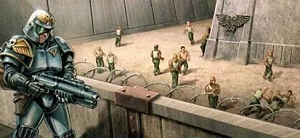
\includegraphics[width=\figwidth]{pics/16/3.png}
	\end{center}
\end{wrapfigure}
The elevator's doors slid shut behind Fumbles and the Inquisitor with an ominous boom, leaving our landing party alone on the pad with the two Deathwatch marines. 
After a few seconds of awkward silence, Aimy pointed out that the Inquisitor was a colossal asshole. 
One of the Marines responded with a vaguely-agreeable grunt, earning him an angry look from his partner (all looks are angry in Power Armor).

The pissier of the two marines tossed Doc in our general direction, and then both of them trained their weapons on our little group and settled into comfortable guard stances. 
All around the pad, the AA guns that defended the facility came to life, and turned to rest on our shuttle well.

We may not have been cuffed, placed in cells, or even properly disarmed yet, but it all-in-all, it was VERY clear that we wouldn't be going anywhere.

Unless someone did something suicidally stupid that is…

Hopefully, it wouldn't have to be us.

\greentext{>The All Guardsmen Party and the [REDACTED] Conspiracy }

\begin{wrapfigure}{O}{\figwidth}
	\begin{center}
		
\includegraphics[width=\figwidth]{pics/16/4.png}
	\end{center}
\end{wrapfigure}
So, to summarize our situation: 
we were sweating through our fancy, but completely unarmored uniforms, on a landing pad, while two bolter-armed Deathwatch Space Marines kept us covered and watched our every movement like genetically engineered super-hawks. 


Since Fumbles was off enjoying the hospitality of the creepily-monotone Inquisitor, our landing party consisted of all us guardsmen, the three adepts, and a very-unhappy Jim. 
Armament wise, none of us except Twitch and Nubby, who had a few party favors crammed into their pockets, were armed with more than our las-pistols. 
We hadn't just left our pulse-weapons behind mind you, we'd just decided to leave them in the shuttle, where their techno-heretical nature wouldn't cause any problems if the Inquisitor running facility had a rod up his ass. 
In retrospect we might've underestimated the size of the hypothetical rod.

Our weapon-filled shuttle was parked a dozen meters away from where the Space Marines had corralled us. 
Aside from our cache of weapons, it was equipped with a multi-laser turret which only Jim knew how to actually use, enough armor to hold off bolter-fire (if the Marines made sure to miss the half-assedly-patched brightlance holes), and MAYBE enough fuel to get us back into orbit. 
Oh, and it also had Sergeant Gravis' stasis unit, but we didn't really see that as tactically significant.

The facility we were on top of was your standard secret mountain base affair. 
You know, a landing pad and a bit of rooftop sticking out of a dangerously steep mountainside, with emperor-knows how much stuff hidden underground. 
Its only real distinguishing features, as far as we were concerned at least, were the local climate, which was blisteringly hot despite the altitude, and the massive ring of anti-air turrets surrounding the landing pad. 
We weren't quite sure who was controlling said turrets or what their reaction time was like, but none of us felt like doing any experiments to figure that out. 


\begin{wrapfigure}{O}{\figwidth}
	\begin{center}
		
\includegraphics[width=\figwidth]{pics/16/5.png}
	\end{center}
\end{wrapfigure}
After our feeble plan to hold onto Fumbles had fallen apart and we'd spent a few minutes stewing in our own juices on the landing pad, the true shittyness of situation began to really sink in.

Aimy started cursing under her breath, and steadily increased the volume until she was ranting like a street-corner preacher. 
Nubby propped his over-sized coat up as a sunshade (no poles were used, the thing was actually filthy enough to stand up on its own, and that was after it'd been washed), and grumpily sat under it, waiting for his voice to return and egging Aimy on as best he could with grunts and gestures. 
Sarge just stood stock-still, muttering darkly to himself and ignoring everyone else, even when Doc tried to ask him for help subduing Twitch, who'd started pacing in circles and ranting about how "he'd known it all along" and "they were ALL in on it".

Really, Tink and Doc were the ones who took it best. 
After an initial freakout, the medic took refuge in the familiar, if difficult, task of tranquing Twitch before he did anything explodey. 
Tink spent a few minutes smugly pointing out that, while we had been arrested by the Inquisition, it HADN'T been for tech-heresy, and therefore everyone owed him an apology. 
He eventually realized no-one was listening and decided to sit down and play with his drone-controller instead. 
There was a tense moment as he drew the controller from his tac-belt, but the Marines eventually accepted Tink's blatant lie about it just being a data-slate, and didn't shoot him.

As for the rest of the party: 
Jim sank down into a little puddle of misery, chattering to himself in binary and rocking back and forth, and the adepts all gathered into a little huddle. 
After a few minutes of serious discussion, the old Diplomacy Adept turned to the rest of us, cleared his throat until we grudging payed attention, and asked us whether we thought Oak had actually turned traitor. 


He seemed surprised by how little we cared.

\begin{wrapfigure}{O}{\figwidth}
	\begin{center}
		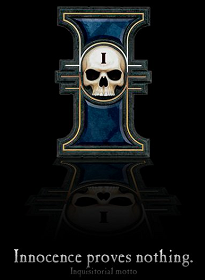
\includegraphics[width=\figwidth]{pics/16/6.png}
	\end{center}
\end{wrapfigure}
I mean, it's not like we thought the question of whether or not our boss was a heretical mastermind that'd been destroying the Inquisition from within wasn't important… We just didn't see how it was relevant to our current situation.

Either:
\greentext{>A: Oak was a heretic. In which case the Inquisition would imprison, torture, and slowly kill us. }

\greentext{>B: Oak wasn't a heretic, but someone had framed him as one. In which case the the Inquisition would probably imprison, torture, and slowly kill us, though they might apologise to Oak about it afterwards if everything was ever sorted out. }

\greentext{>C: Oak wasn't a heretic, and the monotone Inquisitor was lying about the Inquisition ordering his arrest as part of some sort of conspiracy. In which case a bunch of political backstabbers or a shadowy cabal of heretics would imprison, torture, and slowly kill us.}


I'm sure you can see the common theme here.

As far as we were concerned the question of our Inquisitor's moral status was academic, and was therefore something that could be left to the academics while we focused on more important issues. 
Specifically, how we were going to avoid being imprisoned, tortured, and slowly killed.

The old Diplomat got a little huffy with us, and said some very hurtful things about our attention spans and our intellectual capabilities as compared to those of a bunch of a drunken Orks. 
Eventually though, he calmed down and announced his and the other adepts' certainty that Oak was innocent. 
Sarge, who was in just about the worst mood any of us had seen him in, responded with bitter sarcasm, which the Diplomat returned with interest. 
The situation had all the makings of a really good argument, and lacking anything better to do we all gathered 'round to watch the fireworks, but then Tink spoiled everything by asking whether we should tell the Inquisitor everything about the "Zoanthrope" before he finished taking it out of the stasis unit.

\begin{wrapfigure}{O}{\figwidth}
	\begin{center}
		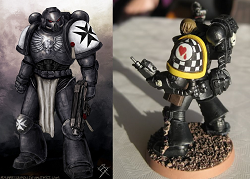
\includegraphics[width=\figwidth]{pics/16/7.png}
	\end{center}
\end{wrapfigure}
Well, you better believe that caught everyone's attention, including the two Deathwatch Marines, who could apparently hear everything we were saying. 
The less-pissy of the two Marines, whose only distinguishing feature was a yellow-edged pauldron with a cartoon heart on it, took a few steps towards us, this paused when he realised his companion wasn't moving. 
The other space marine, who sported a sort of pointy black cross on a white background, just shook his head, and Heart-Marine sheepishly shuffled back to his guard position as we all huddled around Tink's drone-controller.

Spot the Wonder Drone had been incorporated into the Daemonthrope's containment unit when we'd made the thing mobile; 
partially because the drone was as good a central controller for the various systems as anything else we had on hand, but mostly because Fio had REALLY wanted to keep the hunk of wraithbone which suppressed the lion's share of the Daemonthrope's power. 
The wraithbone suppressor had been positioned on the very top of the Daemonthope's pallet, with all its cables and stuff hanging down over the outside of the stasis unit, where they conveniently hid the Daemonthrope's smoky wings from anyone who didn't know to look for them. 
Spot had then been encased in its oversized servo-skull disguise and placed on top of the suppressor, where the drone could easily lift the whole thing off and bring it back with us after the Inquisition had set up whatever they used to contain uppity daemonhosts. 


Anyway, thanks to all this, we had a clear readout telling us that the Deamonthrope's pallet was about a hundred meters below us, and its containment measures were being deactivated by someone who probably didn't know that it held something a just little bit nastier than your average Zoanthrope.

The question was whether we should try to warn them, let them figure things out for themselves, or maybe help things along a little by pushing the big red button on Tink's drone controller.
\begin{wrapfigure}{O}{\figwidth}
	\begin{center}
		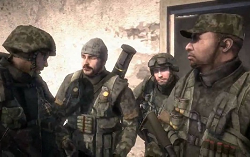
\includegraphics[width=\figwidth]{pics/16/8.png}
	\end{center}
\end{wrapfigure}
The debate over what to do about the Deamonthrope was a very awkward one. 
I mean, you can't just say stuff like "I think we should use this device right here to unleash the daemonhost we brought with us, and then escape in the resulting confusion" in front of a pair of Deathwatch Space Marines. 
It'd be rude. 
Also, they'd shoot us. 
So we had to be careful not to say anything about the daemon, or Spot, or escaping, or anything even remotely related to what was going on really.

Now, if we'd been proper Inquisitorial agents, we'd have used witty metaphors and ironic codewords, possibly leaving the Marines with the impression that we were merely planning a fancy dress party or something. 
Unfortunately we were just a bunch of guardsmen, and had to make do with grunts, shrugs, expletives, and a wide array of rude gestures. 
Judging by the looks on Jim and the Adepts' faces we wound up looking like a bunch of Ogryns trying to argue philosophy, but it honestly worked pretty well. 
Who knows what the Marines thought, maybe that we'd all suffered strokes or something.

Anyway, skipping over a whole lot of nigh-incomprehensible arguing, we eventually decided that the odds of us surviving the Daemonthrope breaking loose were even worse than what we'd get in an Inquisitorial trial. 
Unless, that is, the bug only broke part-way out and they pinned smuggling a Daemonhost into an Inquisitorial facility on us along with everything else. 
Put together, it was enough to convince Sarge that our best option was to fess up to the Daemonthrope's true nature, and hope we got bonus points for saving whichever idiot was in the process of releasing it.

That decided, Sarge stood up, walked towards the Marines until they ordered him to stop or be shot full of holes, told them that Zoanthrope we'd delivered had been possessed by a Daemon, and asked them to warn the Inquisitor not to mess with its containment.

Heart-Marine called him a liar and Grumpy-Marine called him a heretic.
\begin{wrapfigure}{O}{\figwidth}
	\begin{center}
		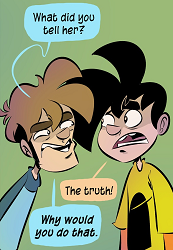
\includegraphics[width=\figwidth]{pics/16/9.png}
	\end{center}
\end{wrapfigure}
Sarge made three more attempts to convince the Deathwatch Marines, but the closest he got to success was briefly arguing with Heart-Marine over whether or not a Tyranid could be possessed by a Daemon. 
That ended with the Marine calling Sarge an idiot for trying to lie about Tyranid biology to a someone who'd fought them for three decades, and Sarge giving up the argument in disgust. 
After that failure, and operating in pure desperation at this point, our fearless leader decided to see if just offering the raw facts to the Marines would work. 
He called Tink over to show them the readouts from the Daemonthrope pallet. 
This resulted in the Space Marines calling the Inquisitor to tell him we had some sort of remote connection to the pallet, and Spot's signal being jammed.

The whole time this was going on, the Diplomacy Adept just stood there, shaking his head and running an increasingly bitter play-by-play critique under his breath. 
When it finally ended with Sarge and Tink both vowing to just stand there and laugh while daemonic bugs killed the Marines, the old Diplomat walked out to Sarge and congratulated him on having learned absolutely nothing during his month of diplomatic tutoring sessions. 
Sarge suggested that the Adept go talk to thee Marines himself if he was so smart, and got told he should have thought of that BEFORE cramming his foot so far into his mouth that he'd started shitting toes. 
After the shocked pause that remark triggered, Doc asked if he could have a turn. 
Both Sarge and Diplomacy Adept told him they didn't care anymore.

\begin{wrapfigure}{O}{\figwidth}
	\begin{center}
		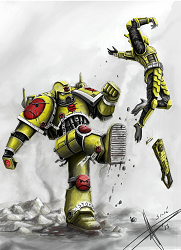
\includegraphics[width=\figwidth]{pics/16/10.png}
	\end{center}
\end{wrapfigure}
So while Sarge and the old Diplomat glared at eachother, and the rest of us began laying plans for taking advantage of the inevitable Daemonthrope escape, Doc walked over to the two Deathwatch Marines and tried to convince them that we totally weren't heretics.

Between the fact that Doc was just about the opposite of a confident and persuasive speaker, and the Deathwatch Marines being a pair of three meter tall killing machines with glowing red eyes and permanent expressions of angry disapproval, the whole thing was rather comically pathetic. 
Our medic stammered and nervously giggled his way through an explanation of how we had no idea what was going on with our Inquisitor or what sort of experiments were going on in this facility. 
We'd just been following what had, at the time, been a perfectly legitimate Inquisitorial order like a bunch of good little guardsmen, and then our Astropath had exploded, and every time we'd tried to get a new one people attacked us, and we'd really had no other option aside from following our original orders, and so on… The whole time both of the Marines just stared at him, as if eyeing a small, furiously yapping dog and debating whether to laugh at it or punt it over the horizon

Doc finally began to run out of steam when he got to the part with the space station, because there was no denying we'd shot, exploded, and MELTED a bunch of loyal Imperial subjects, which is something that's sort of hard to wave off as "just an accident". 
Even if it totally was. 
Also, there was just no way to explain the whole thing with the Warp Fungus without sounding like either a liar or a madman. 
He stuttered to a stop, stared at the impassive Space Marines for a few seconds, and then in a burst of sudden confidence, announced that at least we DEFINITELY hadn't murdered any Space Marines. 
In fact, except for the one that'd gotten skewered by the Hive Tyrant, all of them were still alive, and he could prove it since Sergeant Gravis was currently in our shuttle.

\begin{wrapfigure}{O}{\figwidth}
	\begin{center}
		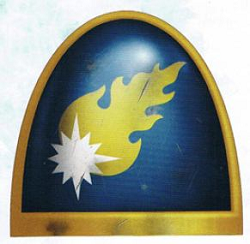
\includegraphics[width=\figwidth]{pics/16/11.png}
	\end{center}
\end{wrapfigure}
Upon hearing Doc's statement Heart-Marine rocked forwards a step, paused for a few seconds to have an inaudible argument with his partner, and then finally told the medic to show him Gravis. 
A minute later they came back out, collected the still-freaking-out Jim, and then wheeled Gravis' stasis unit out onto the landing pad. 
As the two Deathwatch marines huddled over the stasis-chamber and inspected what was left of its occupant, we felt a sudden surge of hope that we could convince them to at least keep the Inquisitor from releasing the Daemonthrope. 
Then Grumpy-Marine spun around, shoved his bolter in Doc's face, and asked why Gravis was imprisoned in a stasis field and what sort of heretical experiments had been planned for him in this facility. 
Doc didn't wet himself in terror, but it was a near thing.

Not being a good bullshitter, our medic-turned-diplomat fell back on the only thing he was certain of: 
the precise details of Gravis' injuries and subsequent treatments. 
The two Deathwatch Marines seemed rather taken aback by the sudden tide of completely incomprehensible medical jargon, and after a few more seconds of glowering they stepped back into their impassive guard positions. 
Doc, having no idea whether this meant they were listing or not, kept on babbling while the rest of us watched and grew more and more antsy. 
Luckily, before any of us ran out of patience and did something to screw everything up again, the third Deathwatch marine arrived.

This Marine was different from the other two. 
In addition to the colorful shoulder-badge (blue with a comet on it) his black armor was decorated with white bits, and he was carrying what even us uneducated guardsmen could recognize as Apothecary tools. 
He came out of the base's elevator at a dead sprint, skidded to a stop in front of Gravis' stasis unit, and began bellowing questions at Doc.

\begin{wrapfigure}{O}{\figwidth}
	\begin{center}
		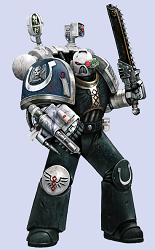
\includegraphics[width=\figwidth]{pics/16/12.png}
	\end{center}
\end{wrapfigure}
As Doc finished his explanation for the second time, the Apothecary turned to the other two Marines and the three of them began arguing. 
They were using their helmet comms, so we couldn't hear a word of it of course, but it was obviously a very heated argument, and since we had a lot on the line (and were bored) we decided to see if we couldn't listen in. 
Approximately half a second after Tink managed to get his drone-controller tuned to their comm frequency and had started working at "cracking it", all three Marines turned to face us and Jim sprinted over. 
The techpriest yanked Tin'ks controller away and suggested that, if we wanted to die, shooting ourselves would be a far more pleasant way to go than getting caught in a half-assed attempt at Aetheric Warfare. 
Tink eventually got his controller back, but only because Sarge promised not to let him use it anymore.

Anyway, the Space Marines resumed their argument after that little hiccup, and after another few minutes of agonizing wait (seriously, it'd been about twenty minutes since we'd received the warning about the Daemonthrope's containment being disabled), they apparently reached a decision. 
The Apothecary announced his intention to temporarily revive Gravis and obtain testimony from him. 
Doc asked how this was possible, Gravis' lungs being rather nonfunctional (see: 
cut in half) in addition to the whole being comatose thing. 
He was told to stop asking questions and be ready to assist as needed. 
Doc had  few seconds to swell with pride at the thought of assisting an actual Apothecary in treatment, and was then nearly crushed as the Space Marine began unloading a hundred kilos of oversized medical equipment onto him.

Everything was laid out, Doc was sprayed with an astartes-grade disinfectant which didn't quite cause him to run screaming in unbearable pain, and the stasis unit was deactivated.

\begin{wrapfigure}{O}{\figwidth}
	\begin{center}
		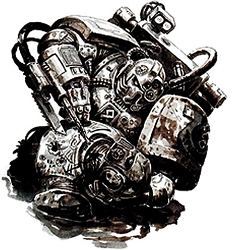
\includegraphics[width=\figwidth]{pics/16/13.png}
	\end{center}
\end{wrapfigure}
The first part of Gravis' revival went about how you'd expect a medical operation being carried out by a centuries-old superhuman to go. 
Afterwards Doc spent something like a MONTH talking about how great a surgeon the Apothecary was, how amazing all the little medical toys he'd used were, and what an honor it had been to be allowed to observe and assist in the operation. 
Even if all he'd been allowed to do was hold a few things (one of which he very-nearly dropped) and dispose of a few vials of bio-toxin (which, lacking a biohazard disposal bin, he just threw off the landing pad). 
Anyway, in a startlingly short amount of time Gravis had been injected, implanted, drained, and a dozen other medical things, and then the Apothecary deftly popped the torso-fied Space Marine out of the Power Armor which had kept him alive for so long. 


I can't really say what we expected the next step of the process to be, perhaps something involving some sort of super-powered stimulants and "blink twice for yes" or something. 
In any case, we certainly hadn't expected the Apothecary to pull out a length of cable, jack one end into his helmet, and the other into one of those weird black sockets on Gravis' spine. 
After that there was a very anti-climatic two or three minutes of watching the Apothecary and Gravis doing nothing, and then the cable was detached, Doc was told to clean up and re-engage the stasis field, and the Apothecary went back to arguing with the other two Deathwatch Marines.

Once again, we stood around like a bunch of pissants, watching a conversation we couldn't hear, but at least it was more interesting to watch this time: 
if their last argument was heated, then this one was practically molten. 
The Marines were actually yelling loud enough for us to hear the occasional word through their helmets, there was a lot of gesturing going on, and the Heart-Marine seemed especially furious about something we REALLY hoped wasn't us.

\begin{wrapfigure}{O}{\figwidth}
	\begin{center}
		
\includegraphics[width=\figwidth]{pics/16/14.png}
	\end{center}
\end{wrapfigure}
When the Marines' argument finally ended with Heart-Marine storming off towards the base's elevator and the Apothecary returning to pick up his medical gear, Doc decided to see if he was allowed to ask questions now. 
It turned out that either the Apothecary was a far friendlier Space Marine than any that we'd met, or perhaps Gravis had said something on Doc's behalf. 
Either way, we were finally given a run-down of the situation.

\greentext{>Sergeant Gravis had testified.}

\greentext{>No, we would not be told how collecting said testimony had worked.}

\greentext{>Because the mysteries of the Black Carapace were not for us to know.}

\greentext{>No, not even if it turned out that we were completely innocent, what part of "not for us to know" didn't we understand?}

\greentext{>No, the secret wasn't that all Space Marines were actually psychic, and our questions-privileges would be revoked if we did not ask about something else.}

\greentext{>Gravis had said we were a bunch of dangerous incompetents, but probably not heretics, and had backed us up in regards to the dangerousness of Daemonthrope, if not the Daemon-ness.}

\greentext{>The Inquisitor had been informed of this, but had been dubious about the reliability of Gravis' testimony.}

\greentext{>After a bit of… debate, the Inquisitor and the Marines had decided that the Daemonthrope would be immediately destroyed. Heart-Marine was going down to observe the procedure. Purely for reasons of protocol, of course.}


The news that they were just going to kill the literally-damned bug, after we'd spent all that time and effort hauling it across the ass-end of the Imperium, did NOT go over well. 
I mean, we probably should've been happy, since it was supposed to be used as evidence of our crimes or something, but still…
\begin{wrapfigure}{O}{\figwidth}
	\begin{center}
		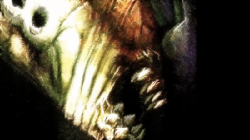
\includegraphics[width=\figwidth]{pics/16/15.png}
	\end{center}
\end{wrapfigure}
Anyway, Sarge made a spirited attempt to convince the Marines that our Daemonthrope-Containment-Unit would work just fine if it was left alone. 
He was told that the Zoanthrope was an abomination in the eyes of the Emperor, and destruction was the only truly safe option. 
Twitch, who was coming back into focus after being tranqued, loudly agreed with that sentiment and was told that he was not being very helpful. 


It then occurred to Tink that it would be very hard to kill the Daemonthrope without removing it from the Containment Unit. 
He asked the Apothecary about this, and was told that standard procedure was to shove the whole thing into a plasma-incinerator. 
Tink asked what would happen to Spot, got asked who "Spot" was, and got as far as "My dr-" before Aimy and Nubby both grabbed him. 
The Apothecary accepted Aimy's explanation that: 
"He named the Containment Unit Spot, he's weird like that" without comment.

It was at that point, as Tink was being dragged away from the marines and quietly being told that Fio could build him a new damned drone if we got out of this alive, that a horribly familiar chittery-scratching sensation went through all of our heads. 
Veteran bug-wranglers that we were, we immediately recognized the psychic screech as a sign of partial containment failure on the Daemonthrope (at least we figured it was partial. 
You know, on account of how there weren't bugs coming out of the walls). 
Sarge immediately informed the two confused Space Marines of the situation, and abandoning all pretenses of diplomacy, demanded to know WHAT THE HELL THEIR BOSS WAS PLAYING AT.
\begin{wrapfigure}{O}{\figwidth}
	\begin{center}
		
\includegraphics[width=\figwidth]{pics/16/16.png}
	\end{center}
\end{wrapfigure}
While Sarge yelled unhelpfully at the Marines, Tink pulled out his drone controller and announced that he'd started getting a faint signal through the jamming again. 
From what he could see, all the regular psi-suppressors were offline, the Wraithbone one had been disabled, so only the stasis field was left keeping the Daemonthrope in check. 
Feeling pretty sure that he knew what his orders would be if he asked for them, the techie immediately started mashing the button to re-engage the Wraithbone suppressor. 
Through some sort of miracle the signal made it through, and the psychic pressure of the Daemonthrope's mind began to diminish. 
For about ten seconds that is, then Spot 2.0 reported a "FLAGRANT SYSTEM ERROR" and a second psychic screech knocked all non-superhumans on the pad to their knees.

Over by the Marines, Sarge and Doc hauled themselves back to their feet and practically begged the Astartes to DO SOMETHING; 
the two Deathwatch Marines ignored them and started arguing again. 
Since our guards were preoccupied, and it looked like the shit was about to hit the fan either way, the rest of us decided this would be a good time to go collect all the weapons that had been left in the shuttle. 
Jim and the Adepts were left standing in the middle of landing pad, viewing the situation with increasing alarm, and were therefore in the best position to observe what happened next.

A third screech doubled everyone over again, and was followed by the "sound" of Fumbles screaming for someone to come help him before "they all go loose". 
Then the entire pad shook and a geyser of fire and blackish-green lightning shot out of the facility's roof. 
As we all pulled ourselves upright and followed the standard Guard post-explosion procedure of asking everyone else if they were dead, the Heart-Marine punched his way through the elevator's doors. 
He began walking towards us, and then turned around as a pair of lightning-wreathed figures rose out of the flaming crater behind him.

\begin{wrapfigure}{O}{\figwidth}
	\begin{center}
		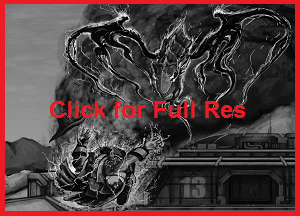
\includegraphics[width=\figwidth]{pics/16/17.png}
	\end{center}
\end{wrapfigure}
The closer figure was a human-looking shape obscured by some sort of blueish energy bubble. 
Judging by the hat and coat it was wearing, plus the fact that the only other nearby psyker we knew of was currently "screaming" for help somewhere down below us, it was probably the Inquisitor. 
There was nothing indistinct about the second figure, it was the Daemonthrope in all its horrible unholy splendor.

The three meter tall snakelike bug still had Sarge's hull-metal shield wrapped around its head, but its eyes blazed red through the metal and a pair of horns, as well as a far more daemonic-looking maw, had somehow formed on the surface of the half-slagged shield. 
The big change though was the wings: 
inside the stasis field they'd been sort of vestigial-looking, but now they stretched twice as wide as the Daemonthrope was tall, and they looked a lot more solid than we'd ever seen then. 
Before this, and when they'd been sported by the possessed Knarloc and the Cogtain, they'd been sort of indistinct and smokey, now they were more like clouds of ink bound into tentacle-like tendrils, and green static crackled through and around them like the field of a poorly-maintained power-weapon. 
All-in-all it was the most daemonic looking thing we'd ever seen, and mind you that list includes a fair few daemons.

As the two of them rose out of the crater in the facility's roof, the lightning arcing between the Daemonthrope and the Inquisitor's shield steadily intensified. 
Just as it occurred to us that we should probably do something to help, the Inquisitor's shield disappeared with a  little pop. 
The man hung there for a second, looking surprised, then let out a terrified scream as the electricity reappeared all along his body. 
His back began to arch, then bend, then crackle. 
There was a final shrill scream, and a horribly gooey crunching sound, and a basketball-sized sphere slightly cooked gore and overly-dramatic clothing splatted to the ground.

\begin{wrapfigure}{O}{\figwidth}
	\begin{center}
		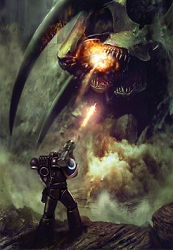
\includegraphics[width=\figwidth]{pics/16/18.png}
	\end{center}
\end{wrapfigure}
Jim and two out of three Adepts screamed, Aimy snickered, Tink and Twitch simultaneously yelled "TOLD YOU SO" at no-one in particular, Sarge facepalmed, and Doc looked up at the Apothecary. 
The medical-marine let out a weary sigh as the Inquisitor's hat drifted down to rest on top of his compressed corpse, and muttered something about needing yet another new Inquisitor. 
Nubby, his voice returning, pointed out "da big daemonic bug fing 'overing over dere", which was entertaining itself by tearing a hole in the fabric of reality, and asked the Marines what they were going to do about it. 
Grumpy and Heart-Marine both let out battle cries and charged forward; 
the Apothecary shook his head and followed them at a more sedate pace.

With a little mutter about them having fun with that, Nubby started to sidle towards the shuttle, only to be yanked into the air by Sarge, who was already bellowing orders and demands for information at the rest of us. 
Jim reported that the shuttle was still out of fuel, still had twenty AA guns pointed at it, and STILL had its long range comm jammed. 
Tink checked his controller and said that his drone was coming back online, and the wraithbone suppressor MIGHT be salvageable if he went down to fiddle with it. 
Sarge digested this, and then declared that, since running away and calling for reinforcements weren't viable options, our only real choice was to kill the bug.

The problem with this idea was that none of us had ANY desire to go toe-to-toe with something that could compress someone into paste with a glance... 
Luckily, there were three crazy bastards in power armor who would do it for us. 
All we needed to do was figure out a way to help the Marines without getting ourselves horribly killed in the process. 
A short debate was held, and by the time the Deathwatch Marines had opened fire, a plan had been formed.

\begin{wrapfigure}{O}{\figwidth}
	\begin{center}
		
\includegraphics[width=\figwidth]{pics/16/19.png}
	\end{center}
\end{wrapfigure}
It was decided that Sarge and Aimy would stay on the surface. 
They'd do their best to assist the Marines, probably by picking with the small tide of Daemonids that'd started pouring out of the newly-opened warp-rift, and try to avoid drawing too much of the Daemonthrope's attention. 


Meanwhile, Tink would go retrieve his drone and the Wraithbone suppressor, and then try to figure out a way to weaponize it, while Nubby would do the same thing with Fumbles. 
Twitch would support them and lend his skills to the whole weaponizing thing, and Doc would go along to make sure nobody did anything retarded, which technically made him the man in charge. 
Doc was not thrilled with this assignment.

Finally, Jim and the Adepts were told to go… do something useful. 
Like getting the AA guns sorted out, or unjamming the long-range comms, or finding some sort of holy artifact stored in a case marked "In case of Daemonic Incursion Break Glass". 
Anything that got them out of the line of fire really. 
They accepted their orders without complaint, and scampered off after Doc's team towards the partially-destroyed elevator into the base.

\begin{wrapfigure}{O}{\figwidth}
	\begin{center}
		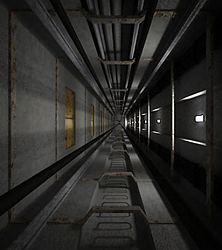
\includegraphics[width=\figwidth]{pics/16/20.png}
	\end{center}
\end{wrapfigure}
Those of us in "Team Doc" climbed through the hole that Heart-Marine had punched through the elevator's doors. 
Inside we discovered the reason for the Marine's violent exit: 
the elevator's car appeared to be stuck about halfway down the shaft and all the lights and control panels were dark. 
There was a maintenance ladder on the far side of the shaft which, judging by the massive hand and foot shaped dents in its rungs, the marine had used to get back to surface. 
We noticed that a few of the rungs had either broken or been ripped entirely out of the wall, but the Space Marine weighed a lot more than us, so we figured it was probably safe and began climbing down. 


Jim and the Adepts were a little more dubious, but they eventually gave up looking for other options and  followed us. 
After Twitch popped a rung loose (which barely missed Doc) and dropped half a level, they decided that whatever they were going to do could probably be done on the first level and hastily exited the shaft. 
We asked them to look into fixing the elevator while they were at it.

The signal from Spot and the volume of Fumbles' periodic incoherent psychic shouts peaked three levels below the stuck elevator, and we decided to exit the shaft. 
Tink suffered a minor heart attack when the first thing he saw after prying open the doors was a pair of turrets aimed at his nose, luckily they didn't seem to register him as a threat, and the rest of us managed to catch the techie as he reflexively dodged backwards into the shaft. 


After a little debate over whether the turrets were "just waiting for us to let our guard down", which ended with Nubby tossing a half-eaten ration bar at one of them to see if they'd return fire, we all climbed through the doors. 


\begin{wrapfigure}{O}{\figwidth}
	\begin{center}
		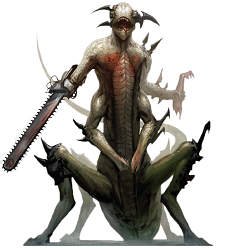
\includegraphics[width=\figwidth]{pics/16/21.png}
	\end{center}
\end{wrapfigure}
We found ourselves in a short hallway that ended with a second pair of turrets and an impressive looking security door. 
Another debate was started over whether the turrets would attack us if we tried to plasma the door open, but Doc resolved the issue by checking the door's controls and discovering that it wasn't actually locked. 
In fact none of the doors we ran into on our way into the base were locked and all the turrets were just as immobile as the AA guns on the surface had been, which was both convenient and disconcerting as hell. 
I mean, we'd just delivered a daemonically possessed Zoanthrope to the place. 
Who knew what sort of shit was penned up down here just waiting for a chance to escape…

Well, actually, the recently-squished Inquisitor had probably known, since judging by the ransacked appearance of the facility he'd been spending the last week or so gathering up everything in the place as evidence of heretical experiments or whatever. 
He was a bit too busy being an asshole (also dead) to share that info with us though. 
Anyway, none of us, not even Twitch, had time to spare worrying about what was in the base or why its security was offline, because we could hear and FEEL the battle going on back up on the pad. 
We followed Spot's signal, rushing through hallways and across recently-stripped rooms without incident, until we finally reached a security door with a piece of paper that said "EVIDENCE STORAGE" taped to it. 
We opened the door, which led to yet another turret-filled hallway, at the exact same instant as some sort of eight-legged, augmetic-covered lizard monster came through the far door.

We looked at the lizard monster, it probably looked at us, something in the room behind it exploded, and then Nubby slammed our door back shut.

\begin{wrapfigure}{O}{\figwidth}
	\begin{center}
		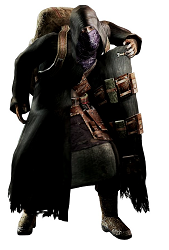
\includegraphics[width=\figwidth]{pics/16/22.png}
	\end{center}
\end{wrapfigure}
A bare second after the door slid closed something slammed into it, leaving a large outward dent in metal. 
This was followed by the sound of four turrets beeping to life and a sort of general fracas as they and the lizard monster sorted out their differences. 
Nubby, his finger still held firmly on the "Close" button, suggested finding another way into the evidence room, or at least waiting to see if the turrets won. 
Doc, feeling like he should do something leadery, announced that there probably wasn't enough time so we'd have to open the door and deal with the thing. 
The rest us agreed, but the question of just how to do it was up for debate.

After a short argument, in which it was decided that trying to flash and rush a creature that had a metal plate instead of eyes and could punch head-sized dents in security doors was stupid, we decided to go with our other usual strategy of blowing the ugly thing up. 
There was a problem with this plan though: 
it'd been several weeks of combat since our last resupply and Twitch's stockpile of explosives down to just his backup-backup grenade and frag mine, plus the single improvised explosive which Sarge had let him bring on the shuttle. 
Twitch asked for the rest of us to pony up whatever we had, but Tink and Doc didn't have anything except a few flashes (Doc was given shit for not saving the syringe of face-melting biotoxin that had been recently extracted from Gravis, at least until he threatened to go get another one and make Tink carry it). 
Nubby, on the other hand, grinned an evil little grin when he was asked, and reached into his perpetually-filthy coat.

Up on the surface, Brother Bellicus of the Black Templars noticed a large group of daemonic hormagaunts moving to flank him, reached for his grenades, and swore when his hand closed on nothing.

\begin{wrapfigure}{O}{\figwidth}
	\begin{center}
		
\includegraphics[width=\figwidth]{pics/16/23.png}
	\end{center}
\end{wrapfigure}
At Twitch's mark Nubby popped door open just wide enough for a lumpy object, which consisted of a half-dozen crosswired lasgun powerpacks wrapped with tape and nails, and two astartes-sized frag grenades to be tossed through. 
A few second later the door was reopened as far as the dent in it would allow, and we all squeezed into a hallway which was a bit worse for wear and smelled rather disturbingly like grilled grox. 
We all resisted the urge to see if the xenos' remains tasted like they smelled, made our way to the far end of the hallway, and discovered that the door had locked itself when the turrets had activated. 
Since said turrets had been pounded to scrap by the lizard-thing, Tink just plasma-ed the door's locking mechanism and opened it to reveal a scene of pure mayhem.

To start with, it wasn't an Evidence Room, it was an Evidence WAREHOUSE. 
The place was absolutely massive and filled with stacks upon stacks of  =][= stamped boxes as well as a few hundred large metal cubes that we guessed were some sort of mobile prison cell. 
The stacks had probably been all neat and orderly up to a few minutes ago, but the explosion that had preceded the Daemonthrope's escape had occurred just on the other side of the room's left wall. 


The crates and cells had been scattered across the room, many of them cracking open in the process. 
Servitors, terrified scribes, prisoners, and escaped xenos specimens were running in every direction, several things had caught on fire, and in the center of the room there was the mother of all three-way melees. 
As far as we could tell the teams were: 
the remnants of ex-Inquisitor's retinue, a group of servitors and prisoners led by something that looked like a human except with the size and musculature of an Ork Warboss, and what we guessed (based on all the extra limbs and such) was an entire genestealer cult.

Nubby tried to close the door again, but was stopped by Doc.

\begin{wrapfigure}{O}{\figwidth}
	\begin{center}
		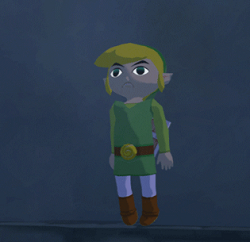
\includegraphics[width=\figwidth]{pics/16/24.png}
	\end{center}
\end{wrapfigure}
We stared at the carnage for a while, and then unanimously decided that we wanted NOTHING to do with any of it. 
Don't get me wrong, we were all brave upstanding soldiers of the Astra Militarum. 
"The Many, The Expendable, the Guard" and all that… It's just that we had more pressing things to deal with, and honestly we just didn't really care about who was fighting who over what. 
In our professional opinion they all looked like psychotic assholes, so we were perfectly fine with them killing each other to their hearts' content, at least so long as they didn't drag us into it.

We began sidling around the edge of the room and towards the Daemonthrope's crater (the Sidle being the form of movement which best conveys "I am not part of this, please ignore me and go about your business/argument/murder"). 
It took a little work to find our way through the scattered evidence boxes while simultaneously trying to keep as much cover as possible between us and the melee, but aside from the occasional stray shot whizzing by or still-warm corpse lying in our path, we managed to avoid most of the locals.

There were only three real interruptions in our progress. 
The first was when a terrified man we recognized as the scribe that had accompanied the Inquisitor on the landing pad nearly ran into us. 
Twitch shot him on reflex, and the rest of us refrained from commenting.

The second interruption was a little more eventful. 
The giant man-thing in the middle of the room bellowed, a cell crashed into the wall ahead of us, and something tentacular began to worm its way out. 
Twitch shot this interruption on reflex too, but this time we all joined in. 
After a few volleys the tentacles retreated into the cell, Twitch tossed his frag grenade in after them, and we continued on our way.

The last interruption occurred as we neared the crater entrance and did not begin with Twitch shooting anyone, but that was only because Nubby grabbed his gun.

\begin{wrapfigure}{O}{\figwidth}
	\begin{center}
		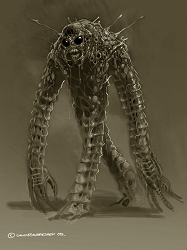
\includegraphics[width=\figwidth]{pics/16/25.png}
	\end{center}
\end{wrapfigure}
As we approached the edge of the crater, three indistinct forms that looked a bit like short cloaked figures came around a pile of crates and practically walked into us. 
Nubby stopped Twitch and gestured at the rest of us to squeeze against the wall. 
We did as he said, and watched in surprise as he cheerfully waved at the three figures then directed them towards the exit. 
There was a greasy croaking sound, a whiff of something absolutely vile, and then the figures just vanished into thin air.

That was a little disconcerting, but Nubby told the rest of us that the it was fine: 
the cloaked whatsits were "Bendies", and they were wonderful people. 
For horrible mutant xenos at least. 
Apparently they hung out in the sewers on some hive worlds and were a great way to get rid of things. 
You know, like proscribed substances that no one would buy, or pieces of equipment that you just happened to have found lying around on the battlefield, but turned out to have belonged to the Commissar and now had your fingerprints all over them. 
Also bodies, great for getting rid of bodies. 
Anyway, wonderful people he said, aside from the smell. 
The rest of us eyed Nubby, who had never intentionally bathed or changed his underwear in his life and whose breath could tarnish ceramite, and decided not to comment.

Shortly after that slightly disturbing encounter we reached the gaping hole that had been blasted in the room's wall. 
The room on the other side was a much smaller version of the evidence room, with a brand new daemonthrope-installed skylight. 
We guessed that it had held fifty or so evidence boxes, one of those mobile cells, and eight-ish Inquisitorial minions. 
Now it was filled with… parts. 


Anyway, the knee-deep gore was just backdrop, what really caught our eyes when we peered through the crater was the only intact thing in the room: 
the top half of our Daemonthrope Containment Unit. 
Oh, and the half-naked woman who was crouched on top of it and singing.

\begin{wrapfigure}{O}{\figwidth}
	\begin{center}
		
\includegraphics[width=\figwidth]{pics/16/26.png}
	\end{center}
\end{wrapfigure}
After an initial second of shock, scantily-clad women being just about the last thing we'd expected to find in an Inquisitorial research facility, we realised that things were not as they seemed. 
It's hard to say what tipped us off exactly, it might have been the odd shape of her ears, or the unnatural harmonics of or singing, or maybe it was the words "ELDAR SUBJECT \#4" printed on the back of her tattered straitjacket. 
Regardless, our well-honed Inquisitorial investigation abilities told us that, while the creature prying at the containment unit was female, she was not a woman. 
She was also not an Ork, no matter what Twitch said.

So no shit, there we were standing in the only entrance of a room containing a half-naked, unarmed Eldar of the female persuasion, who was apparently too focused on singing to the Daemonthrope Containment Unit to even notice our arrival. 
The question of what to do in this sort of situation is something that bored guardsmen (or idle cogitator adepts) might spend endless amounts of time arguing over. 
Not us though, we were above that sort of thing…. 


Yeah, okay, no we weren't. 
I mean, aside from avoiding work and blowing things up, pointless arguments (especially sordid ones) were just about our favorite pastime. 
It was just that before we could get started Tink noticed that a tendril of wraithbone was snaking out towards the singing Eldar from the Containment Unit. 
Before any of us could stop him the techie stepped around the corner, raised his plasma gun, and told the Xenos to stop messing with his stuff and get her own damned Wraithbone.

Nubby snickered, Doc groaned in exasperation, and Twitch pulled Tink out of the way of the bolt of lightning the Eldar flung at him. 
We all reflexively ducked into cover as two more lightning bolts shot through the hole, and when we peeked around the corner again the entire back half of the small room was filled with an opaque mist.

\begin{wrapfigure}{O}{\figwidth}
	\begin{center}
		
\includegraphics[width=\figwidth]{pics/16/27.png}
	\end{center}
\end{wrapfigure}
The next minute or so were spent calling Tink names. 
This was not the most productive use of our time, but none of us were dumb enough to try running into the mist and dislodging the xenos psyker. 
Doc was especially miffed, since his whole job had been to stop the rest of us from doing something like this, and Tink kept using that as an excuse for why this wasn't his fault.

Anyway, after another minute or so of juvenile arguing it became apparent that the Eldar's mist wasn't going to just dissipate on its own and something proactive needed to be done. 
Unfortunately our options were sort of limited. 


Tink proposed a flash and clear, but the rest of us had bad memories of the last time we'd tried that on a prepared psyker, and made it Plan B. 
Nubby spoke up next, and suggested going to get Fumbles, who was still making noise somewhere at the back of the evidence warehouse. 
Since this would involve either splitting up or leaving the Eldar to mess with the Containment Unit, and because we weren't too optimistic about Fumbles' ability to go head-to-head with an Eldar psyker, this was made Plan C. 
Twitch began to suggest something truly harebrained, but was cut off by Doc, who'd decided that he'd had enough and it was time to "Take Charge of the Situation". 


In an odd repeat of the last time we'd faced this sort of thing, Doc poked his head around the corner and attempted to engage the Xenos in diplomacy. 
To our immense surprise, instead of shooting our medic in the head with a lightning bolt, the Eldar stopped singing to listen to him.

\begin{wrapfigure}{O}{\figwidth}
	\begin{center}
		
\includegraphics[width=\figwidth]{pics/16/28.png}
	\end{center}
\end{wrapfigure}
Now, Doc wasn't a good smoothtalker, but he did tend to radiate a sort of awkward earnestness, which can really count for something in this sort of situation. 
The rest of us watched this all with varying degrees of incredulousness as he started off with an apology for Tink's behavior, and then began explaining the overall situation and how the Containment Unit figured into it. 
The Eldar only responded with more silence, but since that wasn't a lightning bolt, Doc took it as a good sign and moved a little farther into the room as he continued talking

It was honestly the most impressive attempt at interspecies diplomacy we'd witnessed. 
I mean sure, we'd seen whole worlds shared between humans and the Tau, but the slit-heads tend to be sort of wishy-washy and there'd probably been a lot of highly trained diplomats involved in all that. 
This was just one slightly naive soldier trying to convince a xenos (who probably had a massive grudge against the Inquisition, not to mention a racial affinity for dickishness) to give peace a chance. 
It was powerful, moving really, and we all honestly believed that given enough time it totally would have worked.

The thing was though, that while Doc was making his heartfelt plea, Tink was playing around with his drone controller and managed to get control of Spot's recon sensors as well as one of the mundane psi-suppressors…. 
And we were sort of on a tight schedule what with the Daemonthrope doing Emperor knew what up above us and Fumbles still needing a rescue… And, you know, better safe than sorry, right?

The Eldar had a second to be very surprised when her cloud of mist fizzled into nothing, and then a barrage of plasma and pulse rounds knocked her off the Containment Unit. 


Doc was NOT happy. 
Even though we pointed out that our shots had missed anything immediately fatal, so if he really wanted to he could patch the Xenos up and give her the whole friendship speech again.

\begin{wrapfigure}{O}{\figwidth}
	\begin{center}
		
\includegraphics[width=\figwidth]{pics/16/29.png}
	\end{center}
\end{wrapfigure}
With that last obstacle out of his way, Tink ran over to the Containment Unit to see what the Eldar had done to it and figure out if the fancy wraithbone suppressor was salvageable. 
While he got to work, Doc grumpily dragged the bleeding xenos into a position where he could simultaneously treat her and keep an eye on the entrance. 
Nubby and Twitch loitered for a few seconds to see if they were needed for anything, until an especially loud shout for help from Fumbles reminded them that they had something better to do.

Nubby and Twitch's trip around the edge of the big room was relatively uneventful. 
It seemed liked everything that was capable of movement had either fled the room or run off to join the big melee, which was now reaching some sort of climax. 
The two troopers ignored the massive clusterfuck, pausing to let the occasional running gunfight go past or dodge a falling stack of boxes. 


The only real excitement was when a cargo servitor holding an obese man crashed across their path, and then began bashing its captive against one of the stacks like an unwanted cat. 
The fat man was probably a psyker, because as he screamed for help reality went a bit non-euclidian and the floor started growing faces, but that might have had more to do with the large box labeled "EXTRA HERETICAL" that he was being bashed against. 
Either way, the two troopers ignored the altercation and walked the through the patch of warped reality with the ease of people who'd seen worse phenomena on trips to ship's mess.

Aside from those little inconveniences, finding Fumbles really wasn't that hard. 
It was just a matter of heading in the general direction of all the psychic shouting, and then homing in on the sense of bowel-loosening fear emanating from the little psyker. 
So before long Twitch and Nubby reached the corner of the room where Fumbles was hiding and discovered what had him so worked up. 
They then very carefully stepped backwards into cover to observe the situation.

\begin{wrapfigure}{O}{\figwidth}
	\begin{center}
		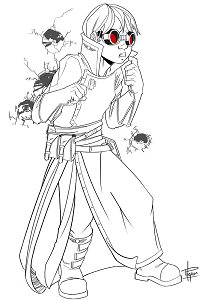
\includegraphics[width=\figwidth]{pics/16/30.png}
	\end{center}
\end{wrapfigure}
The scene was a… weird one. 
Fumbles, or some other scrawny little psyker that periodically flickered in and out of visibility and radiated fear, had been chased up a large pile of boxes by a mob of small, green figures that looked vaguely like Nubby. 
The Gretchins were taking turns climbing up the pile and then fleeing back down as Fumbles' aura of terror overwhelmed them, but that sort of behavior wasn't anything too unusual given their racial affinity for cowardice, it was their boss that was the weird part.

You know those really secure prisoner transport thingies? 
Like with all the straps holding someone to a gurney, along with a facemask and maybe some padlocks? 
Dial that up to 11, replace the gurney with a hand-truck being pushed by three Gretchin standing on each other's shoulders, and replace the prisoner with a raving Ork Weirdboy surrounded by an aura of crackling green light. 
And when I say raving, I mean it. 
The weirdboy could speak gothic, seemed to be using his mouth to compensate for being unable to move anything else, and from the sound of it was (even by Ork standards) completely bat-shit insane. 


It was hard to keep track of everything he was saying, but in the minute or so Twitch and Nubby were listening, the primary theme seemed to be that he wanted Fumbles' head. 
Literally. 
You know, like attached to his shoulder with stitches and stuff. 
He even had a Gretchin with a surgical mask standing by. 
From what we could tell his motivation for this had something to do with two heads being better than one, and it being the secret to "DA BRAINY 'UMMIE'S POWA". 
So yeah, totally nuts, and very frustrated with Fumbles, who kept doing rude things like refusing to come down to be decapitated or claiming that he was only a figment of the Ork's imagination.

\begin{wrapfigure}{O}{\figwidth}
	\begin{center}
		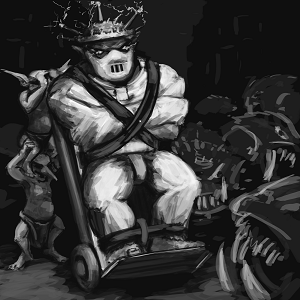
\includegraphics[width=\figwidth]{pics/16/31.png}
	\end{center}
\end{wrapfigure}
Now, as amusing as it would've been to stand there and keep watching the Ork arguing with Fumbles, it just wasn't in the cards. 
Shortly after Twitch and Nubby arrived, the Weirdboy ran out of patience and announced that Fumbles had "TILL DA COUNT OF… UH… FOUR! 
TA COME DOWN, OR IMMA SQUIG YA!"

Up to this point Twitch had just been muttering to himself about how he'd known it all along, and Nubby had mostly been trying to figure out if the box he was hiding behind (marked "PROBABLY NOT HERETICAL") had anything tactically useful and/or valuable inside of it (it didn't), but the this new time limit kicked them into gear. 
Both troopers raised their weapons and got ready to shoot the Weirdboy as soon as it finished its counting and began drawing on its notoriously unstable powers. 
Over the next twenty seconds the Ork (with the help of his Gretchin horde) managed to count up to two, then skipped to five, got confused at eight, went back down to six for another try, and finally decided to skip ahead to thirteen. 
Nubby and Twitch lowered their weapons again.

Since there was apparently enough time to do something more clever than just spraying and praying, Twitch brought out the mechanical-action mine that was his last remaining explosive. 
For his part, Nubby began waving at Fumbles while concentrating on the thought of turning Twitch invisible while he planted the mine on the still-counting Weirdboy. 
Fumbles noticed the waving and caught on pretty quickly: 
the little psyker faded back into visibility, screwed up his face in concentration, and Twitch faded out. 
The demolitions trooper moved fast, which is why he was only five meters from the Weirdboy when a violent burst of energy from the warp smashed into Fumbles' mind, sending him reeling. 
Twitch swore as his invisibility fizzled, hucked the mine towards the Weirdboy like a frisbee, and sprinted back towards Nubby as the little trooper opened fire on full-auto.

\begin{wrapfigure}{O}{\figwidth}
	\begin{center}
		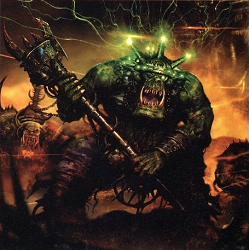
\includegraphics[width=\figwidth]{pics/16/32.png}
	\end{center}
\end{wrapfigure}
Several things happened at once. 
Twitch's mine bounced off the thick metal band restraining the Weirdboy's head, sailed off in a random direction, was snatched out of the air by an overenthusiastic Gretchin, and promptly exploded. 
The force of the blast knocked the Weirdboy's dolly over backwards, taking the Ork out of Nubby's line of fire and crushing the three Gretchins that had been pushing it. 


Nubby adjusted his aim, but as he did so, the ork psyker bellowed something. 
Somewhere in the pack of Gretchins one of them exploded in a shower of green sparks and a small cloud of acrid smoke, the rest surged forwards with a high-pitched "WAAAGH", intercepting Nubby's fire and closing the gap surprisingly fast. 
Nubby held the trigger down until Twitch reached him, then they both did some quick math, decided that thirty-and-an-enraged-weirdboy-to-two odds weren't in their favor, and cheesed it.

Now, despite what it looked like, this was not a cowardly retreat. 
It was actually a carefully planned tactical maneuver to distract the enemy from the true objective. 
Or at least it turned out that way in any case. 
Veteran retreaters that they were, Twitch and Nubby easily outpaced the xenos and broke contact long enough to come up with a plan and split up. 


Twitch stayed on the path they'd been following. 
He found a nice firing position and started shooting Gretchins as they came around a handy corner, racking up seven kills without any real trouble. 
Then the Weirdboy (and the Gretchins pushing him) shot around the corner, tilting up on one wheel, and bellowing "ITZ SQUIGGIN TIME", as he came. 


\begin{wrapfigure}{O}{\figwidth}
	\begin{center}
		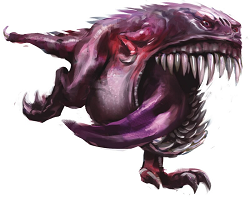
\includegraphics[width=\figwidth]{pics/16/33.png}
	\end{center}
\end{wrapfigure}
There was a brief struggle of wills, at the end of which Twitch's mind was fairly certain that he was actually a hyper-carnivorous ball of teeth. 
Luckily, Twitch's body was harder to convince, and shook off the Weirdboy's attack with no more damage than a few lacerations and a pulled muscle or two. 
The demolitions trooper blinked, realized how close to a fate worse than death he'd just come, and decided it was time to get running again. 
The small orkish horde let out another "WAAAGH" and followed him.

A few dozen meters away, Nubby sidled out through a gap between two stacks of boxes and found himself back where the chase had started. 
A quick scan of the area revealed that a few Gretchin had stayed behind, and were in the process of carrying the still-stunned Fumbles down from his perch on the pile. 
Nubby, not being one to do hard work himself when others seemed were willing to do it for him, pulled out a lho stick and casually waited for the Gretchin to finish before gunning them down. 
Then, his heroic rescue completed, the little trooper wandered over to Fumbles and checked the psyker's status by prodding him in the ribs a few times. 
When this elicited nothing more than a faint groan Nubby, muttering to himself about how he always had to do everything, grabbed one of Fumbles legs and began dragging the psyker back towards the Daemonthrope crater.

Meanwhile, Twitch was barely staying ahead of the Weirdboy, who'd started emitting some sort of brilliant, crackling energy that boosted the speed of it and its minions. 
It really was something out of the paranoid trooper's nightmares: 
Gretchin kept popping out of side-alleys before he could turn into them, and every time he hit a straightaway the Weirdboy's hand-truck gained a little ground. 
The fear just lent Twitch even more speed though, and anyway, he had a plan. 
Mind you, it lacked the large amount of explosives that would make it a GOOD plan in his eyes, but it was still a plan.

\begin{wrapfigure}{O}{\figwidth}
	\begin{center}
		
\includegraphics[width=\figwidth]{pics/16/34.png}
	\end{center}
\end{wrapfigure}
On the outskirts of the minor war occurring in the middle of the evidence warehouse, a group of genestealer cultists finally finished off the Inquisitorial minions that had been keeping them from the cell that contained their master. 
They clustered around the cell door and began hacking at it with their claws and weapons, but paused at the sound of approaching footsteps and turned to face the new threat. 


Twitch came around the corner at a dead sprint, saw the group of mutated cultists, sighted on an alley on the far-right side of their group, closed his eyes, and triggered the under-barrel flash grenade launcher on his pulse-carbine. 
He barreled into the stunned cultists, knocking two aside with his shoulders and nearly tripping over a third, and somehow managed to push his way through them to the alley he had targeted, where he slammed head-first into a crate. 
Twitch reeled backwards, barely dodged a falling crate marked "CLASS-5 FORBIDDEN XENOTECH", and staggered into the alley before any of the cultists could follow. 
Behind him there was a high-pitched "WAAAGH" and the distinctive sound of a warp-propelled hand-truck slamming through bodies like a demented war-chariot.

There was a split second where Twitch worried that he'd under-estimated the Weirdboy's momentum and the xenos would just bowl through the cultists and keep chasing, but then he hear a horrible *schlorp* sound and a bellow of: 
"YOUZ GETS A SQUIGGIN, AND YOUZ GETS A SQUIGGIN, AND YOUS GETS A SQUIGGIN, EVERYONE GETS A ZOGGIN SQUIGGIN." With that, Twitch declared the plan a success, and began working his way towards the Daemonthrope crater. 
After a minute or so he ran into Nubby, who complained that he was tired of dragging Fumbles and insisted Twitch take a turn. 
Fumbles groaned and asked whether he could be carried upright, as the floor was really beginning to chafe.

The three of them arrived back at the crater just in time to see Doc get stabbed in the face.
\begin{wrapfigure}{O}{\figwidth}
	\begin{center}
		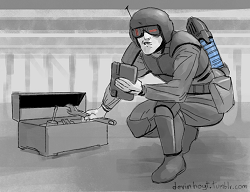
\includegraphics[width=\figwidth]{pics/16/35.png}
	\end{center}
\end{wrapfigure}
Up until Nubby and Twitch's return, things had been pretty uneventful in the crater. 


Tink had started his work by surveying the remains of the Containment Unit. 
It was hard to say exactly what the Inquisitor had been doing to it prior the the shit-fanning, but since the bottom half of it was pretty much vaporized, Tink was willing to bet that it had ended with Daemonthrope doing something to overload the batteries. 
Luckily though, the top half was pretty much intact, and that was where Spot, the fancy Wraithbone suppressor, and a single mundane psi-suppressor had been mounted, so he got to work on prying those free.

While Tink worked he tried to figure out what to do with the stuff once it was pried out. 
His original orders had been to: 
"Go get your Wraithbone thingy and, I don't know, figure out how to turn it into a gun or something.", but he wasn't exactly sure how to do that. 
In fact, he really had no idea how the extra-powerful suppressor worked, and was pretty sure Fio didn't actually know either, despite the little xenos being the one who'd created the thing. 
All Tink knew was that the Tau-thingy made the Wraithbone-thingy project some anti-psi thingy, and if you connected tendrils of psi-conducive material to the device you could spread the anti-psi around a bit.

Anyway, his original plan had been to just pull out Spot, fix anything that was obviously wrong with it and the Wraithbone suppressor, and then maybe make a net or something out of the tendrils. 
The problem was that the tendrils were completely gone, and even worse, the stupid Eldar had done something to stretch the wraithbone out like taffy. 
What had once been a cinder-block sized brick, was now a vaguely phallic-looking object about a meter long, and while Fio's device was still intact, it no longer fit properly. 
Lacking any real idea what to do, Tink decided to just go ahead with the pulling and fixing, and just hope that he'd spontaneously think of something clever.

\begin{wrapfigure}{O}{\figwidth}
	\begin{center}
		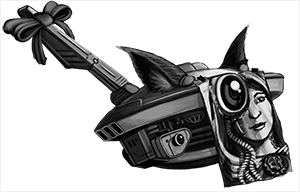
\includegraphics[width=\figwidth]{pics/16/36.png}
	\end{center}
\end{wrapfigure}
Tink still hadn't thought of anything by the time he'd finished prying everything loose, so he screwed around for a few minutes setting up the mundane psi-suppressor next to Doc so the medic would stop bugging him about it. 
While he did this, the techie debated pulling out his plasma gun and telling the Eldar to return the wraithbone to its original shape or die. 
Doc was against the idea for various reasons, and there was a brief argument which ended with Tink asking the highly inappropriate question of why the xenos had reshaped the wraithbone into an, ahem, "giant stone dong". 
Doc impatiently told the techie that she was probably making a spear or something, and suggested that he get back to work.

Doc's response triggered something in Tink's imagination and the techie got thoughtful. 
Then he got even more thoughtful. 
Then he went over to his drone, lined up all the parts in a new orientation, and started snickering. 
And that's why, at the end of things, it turned out that our secret anti-Daemonthrope weapon was Spot the Wonder Drone with an amusingly-shaped wraithbone spear strapped to its undercarriage. 
You know, like a battering ram, or a bayonet, or… well… a lot of other non-phallic things…

ANYWAY, Tink got to work strapping things on and just bending the shit out of Fio's device until it fit the new shape, and the whole time this was going on, Doc continued watching the door and working on his patient. 
The medic's time at the bottom of the crater was even less interesting than Tink's, for the most part at least. 
The Eldar wasn't in great shape: 
plasma and pulse rounds are nasty enough when you're in full armor, taking a barrage more or less naked is NOT good for one's health. 
Still though, they were the sort of wounds Doc was good at treating, and he did a fair job of patching her up. 
Hell, he even cleaned the all the gore and the debris off the area of floor he was operating on, if that's not quality service, I don't know what is.

\begin{wrapfigure}{O}{\figwidth}
	\begin{center}
		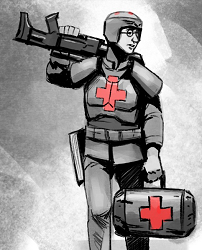
\includegraphics[width=\figwidth]{pics/16/37.png}
	\end{center}
\end{wrapfigure}
Doc did good work. 
Half-cauterized wounds were sprayed with sealant, the two bags of Inquisition-Torturer™ Brand Xenos Blood Substitute (Non-fatal to over 60% of humanoid xenos scum! 
Extend your torture experience for WEEKS!) were administered, a completely-mangled arm was removed and tossed into a corner somewhere, and a bunch of other boring medical stuff was done.

For the most part the Eldar just laid there unconscious, but after a while she started twitching and emitting a bit of random psychic noise, which was distracting enough that Doc asked Tink to rig up the regular psi-suppressor nearby. 
That was it as far interruptions from his patient, but there were also three or four occasions where Doc had to drop his bandages and pick up his weapon. 
Honestly, these interruptions weren't much more interesting than the medical procedures. 
Most of the time it was a matter of something poking its head around the edge of the hole in the wall, and then scampering away after Doc sprayed a bit of suppression fire in its direction. 
The only times when it didn't work like that was when a lucky shot took the head off something that might've been a small kroot hound, and when a heavily armored, but armless, servitor plodded through Doc's fire without seeming to notice, looked around for a few seconds while he reloaded, and then walked away again. 
So yeah, things were pretty dull for Doc, right up until his patient woke up that is.

You know how in stories the beautiful female patient will wake up, meet her doctor's eyes, then smile and say something about how she must be dreaming? 
That didn't happen. 
Doc looked up at the sound of approaching footsteps and set aside his scalpel in favor of his carbine, but relaxed when he saw it was only Nubby and company. 
When he looked back down the scalpel was in his patient's one remaining hand, and it was darting up towards his eye.

\begin{wrapfigure}{O}{\figwidth}
	\begin{center}
		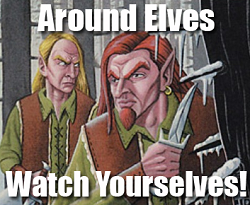
\includegraphics[width=\figwidth]{pics/16/38.png}
	\end{center}
\end{wrapfigure}
Luckily, Doc was a combat medic, which meant he typically treated guardsmen, armsmen, and other violence-prone individuals, and when that sort of person is hurt and confused, they tend to lash out. 
Over the course of his career he'd had his arm broken, been jabbed in the thigh with a fistful of tranq ampules, received small caliber bullets to the chest and helmet, and had been socked in the face at least two dozen times. 
That sort of experience builds up some serious reflexes, so when the wounded Eldar tried to stab Doc in the eye with his own scalpel, the medic was flinching backwards and raising his arm to block before he'd even registered what was happening.

Of course an unarmored arm can only do so much to stop a blade. 
The scalpel went right through Doc's forearm (between what he still referred to as "the inside arm-bone" and "the outside arm-bone"), then continued upwards into the meat of his face, and finally lodged his cheekbone. 
Doc swore and reeled backwards with his arm pinned to his face, but that was still a lot better than getting stabbed in the eye.

The Eldar followed her attack up with a grab for Doc's pulse-carbine, but it was still on its strap and Doc's pinned arm was in the way. 
Doc swore again as the gun caught on his arm and twisted the scalpel in face, and countered by punching the uncooperative xenos in the nose with his free hand. 
This was enough to knock her backwards, but she kept her grip on the gun as she fell and Doc swore a third time as he landed face-and-scalpel first on the ground. 


At this point the Eldar decided that a change of plan was called for. 
While Doc struggled to roll over and bring his gun to bear, she staggered to her feet, sighted on the psi-suppressor that had been set up nearby, and sprang towards it. 
She got to within a meter of it before Nubby and Twitch shot her in the back.

\begin{wrapfigure}{O}{\figwidth}
	\begin{center}
		
\includegraphics[width=\figwidth]{pics/16/39.png}
	\end{center}
\end{wrapfigure}
Nubby and Twitch kept their guns on the prone Eldar as they entered the smaller evidence room. 
Behind them Fumbles, who'd been unceremoniously dumped on the ground as they grabbed their weapons, complained that his nose felt like it was broken, he told to put his big boy pants on. 
At the other end of the room Tink asked if they had everything under control, and then, without waiting for an answer, dropped his gun and went back to working on his drone.

The two troopers advanced past Doc, who'd finally gotten back upright, but still had his arm pinned to his face, and stopped a few meters from the Eldar. 
By unspoken agreement Twitch kept his weapon raised while Nubby moved forwards, hooked a metal toe under the groaning xenos, and flipped her over. 
The Eldar flopped upright with a hacking cough and a groan, Nubby cheerfully told her it served her right for moving around so much after surgery. 
He went on to tell her that she was being very uncooperative, but if she promised to apologize, he was sure Doc would patch her up a second time. 
The Eldar spat blood at him and stated that she would rather die. 
Nubby and Twitch looked at each other and shrugged.

\greentext{>"Well, you 'eard da lady."}


The Eldar's eyes went wide and she got as far as "Wai-" before Twitch and Nubby fired.

\begin{wrapfigure}{O}{\figwidth}
	\begin{center}
		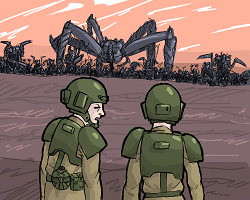
\includegraphics[width=\figwidth]{pics/16/40.png}
	\end{center}
\end{wrapfigure}
Over where he was working Tink let out a surprised curse, and began loudly complaining that there were bits of brain all over Spot's new external battery unit. 
Nubby just snickered, but Twitch yelled some rude things back at the techie and began loudly complaining about how no one was ever grateful. 
When Doc told him to calm down, the demolitions trooper rounded on him and asked whether he was going to start whining about shooting his new xenos girlfriend. 
Doc pulled his arm forwards off the scalpel with a squeching sound, and gingerly poked at the surgical implement stuck halfway into his face. 
He then let out a pained sigh and pointed out that he already had a girlfriend, and he wasn't inclined to feel too sorry for anyone who stabbed him in the sinuses. 
Further discussion was called off on account of the deafening sound of two dozen AA guns opening fire above us, and the arrival of the Daemonthrope at the top of the crater.

The Daemonthrope's arrival was accompanied by a painful wave of psychic pressure and a slight breakdown in the fabric of reality. 
Up at the top of the crater, the walls and ceilings nearest the Daemonthrope sprouted a film of pinkish-green stuff that might've been a cross between flesh and fungus. 
Down at our level the pureed remains of the Inquisitor's retinue began to bubble and reform into the mutated forms of rippers and gaunts.

It was abruptly and unanimously decided that it was time to abandon the room and retreat to the larger warehouse. 
Doc stopped poking at his face, and he, Nubby, and Twitch began firing on the forming daemonids in controlled bursts. 
Tink gathered up his drone and the few tools he still needed, and then sprinted for the exit while the rest of us gave covering fire. 
Fumbles met him at the edge of the warehouse, helped him unload, and then began assisting the techie by providing tools as needed and without being asked. 
Tink didn't actually notice him doing this, but it really was quite helpful.

\begin{wrapfigure}{O}{\figwidth}
	\begin{center}
		
\includegraphics[width=\figwidth]{pics/16/41.png}
	\end{center}
\end{wrapfigure}
A few seconds after Tink had exited, the rest of us slowly fell back. 
As we moved we spared a few glances up towards the Daemonthrope, and were incredibly relieved to discover that it was staying put at the top of the crater. 
We guessed that it had just moved there to get away from the AA guns we'd heard, and was perfectly happy hovering there and shooting lightning bolts at whoever was pestering it up on the surface. 
We wished whoever it was luck, finished our retreat to the warehouse, and set up firing positions around the hole between it and the crater.

Once we were in position it was just your typical desperate holdout against ravenous alien invaders. 
You know, that thing that practically defines life in the guard? 
I won't say it was a stroll through the park, but it really wasn't that hard, even with the Daemonthrope pressing on our minds and the way the dead daemonids kept reforming. 
Of course, things became slightly more difficult when Fumbles jogged over and said Tink needed all of our laspistol power packs and at least four pulse-carbine packs.

Over at his new workstation Tink had put the finishing touches on Spot. 
After the arrival of the Daemonthrope he'd decided that he really didn't need ALL of the mounting brackets he'd been planning to install, and the weird readings from Fio's suppression device could probably just be ignored. 
All that was really left to do was rig up a way to get enough power to the suppressor while still leaving Spot enough to fly, but there was a shortage of heavy-duty batteries, so he'd had to rig up something a little more creative. 
Hence the need for the power packs.

After a little bit of whining and arguing, Fumbles returned with the packs (leaving Doc, Nubby, and Twitch with only five remaining between them). 
Tink slotted them into place, hoped really hard that he'd done the power conversion math correctly, and hit the "On" button on his controller.

\begin{wrapfigure}{O}{\figwidth}
	\begin{center}
		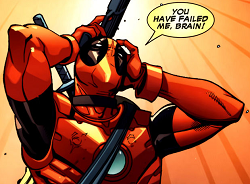
\includegraphics[width=\figwidth]{pics/16/42.png}
	\end{center}
\end{wrapfigure}
First the lights came on, then the hover unit engaged and the stealth field cycled, and finally there was a flicker of static all along the protruding wraithbone *ahem* prow. 
Tink held his breath, then let it out in a high-pitched shout of victory as the oppressive force of the Daemonthrope's mind vanished. 


Over at the hole the rest of us were  little too busy conserving ammo and holding the bloody line to see what had Tink so excited, but we figured it out when Spot shot between us and cut a small swathe through the approaching swarm with its mere presence. 
We cheered as well as the drone did a short victory lap and pushed forward to watch as it rose up towards the Daemonthrope.

Spot the Wonder Drone flashed upwards, sliced through the crackling green shield surround the Daemonthrope, and slammed into the thing's underbelly. 
As Spot's psi-suppressor, er, penetrated the creature's hide, it let out a roar of unfathomable pain and fury, its shield vanished, and the daemonid minions around us collapsed into goo. 
We all cheered again and watched, the inky black tendrils holding the Daemonthrope aloft twisted, flickered, and then… reappeared. 


\begin{wrapfigure}{O}{\figwidth}
	\begin{center}
		
\includegraphics[width=\figwidth]{pics/16/43.png}
	\end{center}
\end{wrapfigure}
We stood there, waiting to see what would happen next, and then flinched when the Daemonthrope let out a roar and fired a bolt of green lightning at someone on the surface. 
Nubby swore, Twitch groaned, Fumbles started whimpering, and Tink asked if anyone could see what was happening to Spot. 
Doc remained calm though. 
The medic looked at the rest of us, and then in a stuffy voice (because he STILL had that damned scalpel in his face) said:

\greentext{>So… unless someone has a better plan, I say we shoot it until we're out of ammo, and then run away if that doesn't work.}


None of us did, of course, so we all gathered together, opened fire, and hoped like hell that the Daemonthrope didn't have much juice left in it. 
As we fired, we couldn't help but notice that only one person up on the surface was firing with us, and they weren't using a pulse weapon.

Up on the surface, Sarge pulled the pin on the astartes-sized krak grenade he'd "borrowed" and hoped like hell this was going to end better than the last time someone had tried it...

\begin{wrapfigure}{O}{\figwidth}
	\begin{center}
		
\includegraphics[width=\figwidth]{pics/16/44.png}
	\end{center}
\end{wrapfigure}
The fight on the top of the facility had begun with the three Deathwatch marines charging forwards in an attempt to blitz the Daemonthrope. 
In the opinion of (possibly former) Interrogator Greg Sargent, this was a very stupid idea.

It wasn't that blitzing a Zoanthrope was a bad idea in and of itself. 
In fact if you look them up in the Tactica, they're defined as "Psychic Artillery" and the preferred methods for dealing with them are generally the same as other varieties of artillery. 
Ideally you just call in an airstrike, or some (preferably longer ranged) artillery of your own, but if that's not an option then you're going to want to get in close where their big guns can't easily get at you. 
Of course the tricky part is not getting blown to little pieces while you close the distance, but the Tactica has some good recommendations there too: 
If you're a Brave Soldier of the Imperium, then you're supposed to just sprint across the killing field, firing wildly and relying on your faith in the Emperor to protect you. 
If, on the other hand, you're a cowardly dog not fit to wear the Emperor's uniform, then you'll want to make use of cover and sneak around the flanks while all the Brave Soldiers get themselves killed.

So, given that Space Marines are the very definition of Brave Soldiers of the Imperium, (and were wearing enough power armor to survive that sort of foolishness) their choice of attack was tactically sound. 
Or it would have been, IF THEY WERE ACTUALLY FIGHTING A ZOANTHROPE.

Seriously, it wasn't some frail, slow-moving creature that relied on distance and minions to protect it from harm. 
IT. 
WAS. 
A. 
DAEMONHOST. 
You know, those things that can turn frail little cultists into nigh-indestructible killing machines capable of tearing tanks apart with their bare hands? 
What the Marines thought they were going to accomplish by getting closer to it was a mystery, especially since it was currently flying fifteen meters over the top of a deep crater.

\begin{wrapfigure}{O}{\figwidth}
	\begin{center}
		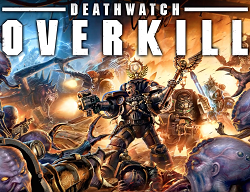
\includegraphics[width=\figwidth]{pics/16/45.png}
	\end{center}
\end{wrapfigure}
Despite the temptation, Sarge and Aimy didn't stand around critiquing the Marines' choice of tactics. 
This was partially because the situation was too serious to waste time being petty and unhelpful, but mostly they just figured the Daemonthrope would handle it for them. 
The two of them slowly advanced behind the Marines, placing aimed shots into the growing number of daemon-tyranid hybrids pouring out of the hole in reality the Daemonthrope was tearing, and waiting to see what was going to happen.

Surprisingly though, what happened was… nothing. 
The three Astartes charged in (well the Apothecary just jogged), spraying fire and fending off the odd daemonid, but the Daemonthrope just manifested a greenish-black shield and ignored them while it poured more and more juice into the widening hole in reality. 
Between shots, Sarge and Aimy snickered to themselves as the Marines reached the edge of the crater and then milled around trying to figure out how to respond to being dismissed as non-threats.

Of course the Deathwatch Marines didn't waste too much time standing around. 
The trio of superhuman warriors drew upon all their centuries of tactical knowledge, and came to the conclusion that they should try shooting the big psychic bug HARDER. 
As Guardsmen, Sarge and Aimy wholeheartedly approved of this decision, and concentrated on keeping the smaller bugs in check while the Space Marines poured a ludicrous number of bolt rounds into the shield.

Seriously, when I say ludicrous, I mean it. 
All three marines were firing their bolters on full-auto (the Heart-Marine was actually using his one handed while firing a Plasma Pistol with the other!), and they were reloading faster than seemed physically possible. 
How much ammo the marines had (or where in the Emperor's name they were keeping it all) was a bit of a mystery, but they Sarge and Aimy both swore that the trio managed to put upwards of two-hundred rounds into the Daemonthrope's shield before it popped.

\begin{wrapfigure}{O}{\figwidth}
	\begin{center}
		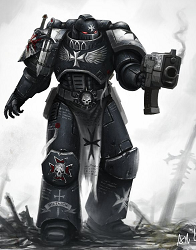
\includegraphics[width=\figwidth]{pics/16/46.png}
	\end{center}
\end{wrapfigure}
Now this is where the Deathwatch Marines learned the real difference between a Zoanthrope and the unholy creature we'd hauled across the galaxy. 
When their barrage broke down the Daemonthrope's shield, it didn't fall over dead or try to wriggle away. 
No, all that a dozen bolt-rounds to the center of mass managed to do was make the thing angry, and daemonhosts can get very, very angry.

The only reason the Astartes weren't vaporized was their superhuman speed and the fact that, despite their initial choice of tactics, they DID have a bit of self-preservation instinct. 
When the Daemonthrope rounded on them, the three Marines scattered, barely avoiding a psychic tantrum that turned roughly fifty meters of facility roof into a warp-tainted mixture of rubble and molten slag. 
Sarge and Aimy watched the light show, noting the power of the attacks and the way bits of dead daemonid rose into the air to fill in the Daemonthrope's bolter-wounds, and congratulated themselves on their decision to stick to shooting the little bugs.

Eventually though, the Daemonthrope's tantrum ended and the bug turned back to its now-shrinking portal. 
It seemed to go pensive for a few seconds, and then with a flap of its wings, the bug entered the portal and its oppressive psychic presence vanished. 
Sarge and Aimy stayed in their cover waiting to see what horrible thing would happen next, but after a solid minute of nothing, they went back to picking off the daemonids.

A few minutes later the last of the bugs were dead, the Marines had clawed their way out of the rubble at the edge of the destroyed area, and everyone was gathered around the shrinking the warp-portal. 
As the hole finally disappeared with a little pop, Sarge sighed in relief, then froze as Grumpy-Marine said:

\greentext{>Hmm, more power than I expected, but far less courage. That was almost too easy.}


 Aimy got as far as "YOU JUST HAD TO FUC-" before the nearby mountaintop exploded in green light.

\begin{wrapfigure}{O}{\figwidth}
	\begin{center}
		
\includegraphics[width=\figwidth]{pics/16/47.png}
	\end{center}
\end{wrapfigure}
The green light was followed by the familiar psychic screeching and the appearance of a rift in reality large enough to peek over the top of the mountain. 
Sarge sighed and facepalmed, while Aimy decided it was time to boost morale via friendly insults, specifically ones targeted at the Grumpy-Marine and "whatever retarded chapter of retards spawned your retarded ass." The black-and-white Space Marine didn't seem to take these completely innocent comments very well, but before anything could come of it both Sarge and Aimy were yanked off their feet.

The Apothecary and Heart-Marine tucked the two guardsmen under their arms like fussy children and began running up the mountain at a pace that could be described as "terrifying". 
Sarge, possibly because he was far less of an asshole, was carried facing forwards, which meant that he was able to watch as the mountaintop grew a layer of flesh-fungus and a tide of mutated gaunts poured over it. 
He briefly considered picking a few of the bugs off while the Apothecary ran, but gave up after an especially large jump jammed his carbine's scope halfway into his eye socket. 
Aimy just swore at the Heart-Marine and promised terrible vengeance for such undignified treatment.

The ride ended when the first of the Daemonids came into range. 
Sarge was placed on a boulder with a good view of the bug-covered slope, Aimy was unceremoniously dumped onto the ground, and the three Deathwatch Marines began advancing towards the glowing mountaintop.

\begin{wrapfigure}{O}{\figwidth}
	\begin{center}
		
\includegraphics[width=\figwidth]{pics/16/48.png}
	\end{center}
\end{wrapfigure}
Once again, it was a matter of Sarge and Aimy providing covering fire while keeping their heads down, but this time the rough terrain and large number of hostiles meant the Astartes' attack was more of a slog than a blitz. 
Not that the lack of speed made it any less impressive, these ARE the Emperor's Angels of Death we're talking about. 
All three of the Deathwatch Marines collected more kills that Sarge while simultaneously dealing with enemy attacks and climbing a bloody mountain. 
If it weren't for the fact that Aimy's sniping skills, not to mention her techno-heretical armament, managed to keep her in the lead on points, Sarge might've had to admit that honest Guardsmen couldn't compete with genetically engineered supersoldiers.

Anyway, the advance to the top of the mountain went off with only two or three sketchy moments. 
The worst of which was when the Grumpy-Marine let himself get flanked by a bunch of mutated gaunts for some reason. 
I mean seriously, he just stood there like an idiot pawing at his belt, it was like he forgot how many grenades he had or something. 
Aimy had to pull off an absolutely amazing barrage of double-kills to keep his stupid ass bug-free. 


 Aside from that, the time when one of the larger Daemonids almost managed to sneak up on Aimy before Sarge noticed it, and the incident with the looser-than-expected boulder, the advance to the mountaintop went smoothly. 
Of course, you know what Murphy says about attacks that go really well…

\begin{wrapfigure}{O}{\figwidth}
	\begin{center}
		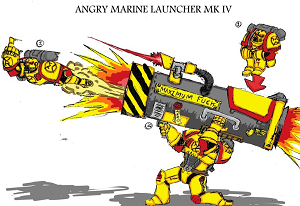
\includegraphics[width=\figwidth]{pics/16/49.png}
	\end{center}
\end{wrapfigure}
Okay, well, technically what happened wasn't an ambush, so maybe the old adage isn't perfect, but the end result was about the same.

The top of the mountain was a smallish plateau with a bunch of sciency antennas on it, plus a growing rift in reality and an irritable Daemonthrope. 
The three Deathwatch Marines advanced right up to the edge of it, cleared out a last wave of gaunts, and then all three prepped krak grenades and vaulted up over the lip of the plateau. 
Neither Sarge or Aimy could see what happened next, but at least one of the grenades must have stuck its target, because the Daemonthrope let out a mind-rending screech of pain. 
Unfortunately, it also let out a blinding blast of green energy which shook the entire mountain, guardsmen included, like an abusive nanny.

Sarge wound up lying on his back, blinking and trying to remember what he'd been doing, and then flinched as something large flew a few meters over his head. 
He reflexively turned and watched as the object sailed a few dozen more meters, clipped a boulder, cartwheeled up in a short arc, landed with a crunching sound, and finally skidded to a halt. 
Sarge blinked again and idly wondered why the unidentified crashing object looked so familiar. 
Then his dazed brain kicked back into gear, put two and two together, got five, decided that was close enough, and signaled his mouth.

\greentext{>HOLY SHIT IT'S RAINING SPACE MARINES!}


Aimy, who was even more out of it than Sarge, moaned and crawled into cover underneath a nearby boulder. 
Not because she understood a single word of what Sarge had said, but because taking cover was the Guard-issued response to confusion and incoherent orders. 
She huddled there for a second, clutching her head and wondering why she'd ever left her regiment, and then registered what Sarge had said at about the same time as the dazed noncom realized it himself. 
Both of them jumped to their feet and ran downhill towards the crumpled form of the Marine formerly known as Grumpy.

\begin{wrapfigure}{O}{\figwidth}
	\begin{center}
		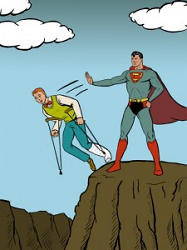
\includegraphics[width=\figwidth]{pics/16/50.png}
	\end{center}
\end{wrapfigure}
Actually the "former" was premature, when Sarge reached the battered Marine he was still breathing and in possession of over three quarters of his appendages. 
It was hard to say whether the missing foot was due to the blast, the fall, or the pack of daemonic rippers that had started gnawing at the Astartes while Sarge was staggering around, but it's not like it really mattered. 
After some initial clearing, Aimy began picking off all nearby bugs, while Sarge propped the wounded Space Marine up against a cover-providing rock and tried to decide what to do next. 
His thought process was interrupted when the rock exploded.

For the second time in five minutes, Sarge found himself on his ass, wondering what the hell was going on. 
This time though, the sight of the Daemonthrope drifting down the mountainside shook him out of it. 
He staggered upright and analyzed his current situation with the speed of the truly desperate. 


It was a complex tactical situation. 
Sarge was bleeding, slightly burned, and had at least one broken rib. 
The Space Marine was still unconscious, and was now slightly less than three-quarters-intact. 
Both of them had been flung a few meters down the scree slope, and were now at the top of a twenty-ish meter cliff. 
Friendlies-wise, Aimy wasn't anywhere to be seen, and neither were the other Deathwatch Marines. 
As for hostiles, all the little bugs in the area were dead, but the Daemonthrope appeared to focused on the wounded Marine, and was gathering greenish-black electricity for another attack. 
Finally, the only option for cover was a smallish pile of rocks a few meters away, which was way too far to drag a tonne of power-armored Space Marine.

It was a tricky situation. 
In fact it was the sort of tactical problem that a tribunal of senior Inquisitors might spend an entire day and a half arguing over...

Sarge didn't have that sort of time though, so he responded to the complex tactical situation by pushing the Space Marine off the cliff.

\begin{wrapfigure}{O}{\figwidth}
	\begin{center}
		\includegraphics[width=\figwidth]{pics/16/51.png}
	\end{center}
\end{wrapfigure}
Despite the apparent retardation of this plan, it worked. 
The wounded Space Marine flopped over the edge a bare second before the Daemonthrope's attack hit. 
Instead of being blown to pieces by a bolt of green lightning, the wounded Space Marine merely suffered a bone-shattering fall and downhill tumble. 
This was unquestionably a win, unfortunately Sarge wasn't in much condition to appreciate it, because it'd taken him just a little too long to shove the heavy Marine over the edge.

The blast caught Sarge in the back as he scrambled for cover, inflicting a few more shrapnel wounds and superficial burns in addition to knocking him prone. 
He struggled back to his feet as the Daemonthope screeched in rage and, deprived of its original target, turned its metal-covered face towards Sarge. 
The dazed noncom attempted to stagger the rest of the way into cover, realized he'd never make it in time, and raised his carbine instead. 
He got off only three shots before the Daemonthrope's eyes flared. 
An invisible force ripped the gun up and out of Sarge's hands, and then began inexorably pressing in on him from all directions…

It was at this point that Aimy decided it was time to stop sitting around waiting for the Marines to show up, and do something heroic. 
Over the last minute or two she'd picked herself up from where she'd been thrown, found a nice firing position, and watched the Daemonthrope's attack in a desperate attempt to discover some sort of weakness. 
Unfortunately, it seemed to lack any giant glowing weak points, and while it had initially sported some nasty-looking wounds on its front, he remains of several daemonids had risen up and filled in the holes in thoroughly disgusting fashion. 


So, lacking any ideas for how to kill a continuously regenerating creature that shrugged off bolt-rounds and grenades, she settled for shooting it in the eye and hoping it was easily distracted.

\begin{wrapfigure}{O}{\figwidth}
	\begin{center}
		\includegraphics[width=\figwidth]{pics/16/52.png}
	\end{center}
\end{wrapfigure}
The Daemonthrope screeched and released Sarge as the pulse-round punched through the metal plate welded to its face and put out its left eye. 
It then turned towards Aimy and then turned and caught a shot in its other eye. 
As Aimy had suspected neither shot did much to incapacitate the creature, but they sure as hell pissed it off.

The rock that the Markswoman had fired from exploded in a shower of semi-molten shrapnel, but by that point she'd already rebased. 
Aimy popped up from her new position, landed yet another headshot, and then scrambled backwards over a ridge of scree, where she paused for a second before picking out another good-looking rock. 
She scrambled downhill, keeping the small ridge between her and the enemy, until she reached the rock, where she readied her rifle for another shot. 
It was then, as Aimy rose up for her third attack, that she realized it'd had been really, really stupid to assume the Daemonthrope would keep hovering around a few meters above ground level while it chased her. 


Aimy peeked out of cover to find the Daemonthrope a mere thirty meters above and in front of her, and with a corona of green electricity already gathered around it. 
The Markswoman reflexively flinched downwards, but it was already too late. 
There was a flash of green light, a blast of heat, and then… nothing.

Finally, after what seemed like an eternity of silence and darkness, there came the horribly, horribly familiar pain.

A couple hundred meters away, Sarge paused his search for his dropped carbine, and listened in confusion to what sounded like the bellowing of a stuck Grox. 
Then after a few seconds the incoherent screaming transitioned into a wail of: 
"WHY IS IT ALWAYS THE FUCKING FACE". 
Sarge gave up the search for his weapon, drew his laspistol, and started sprinting.

\begin{wrapfigure}{O}{\figwidth}
	\begin{center}
		\includegraphics[width=\figwidth]{pics/16/53.png}
	\end{center}
\end{wrapfigure}
Fortunately, Sarge didn't get a chance to try attacking a daemonically possessed Tyranid psyker with nothing but a laspistol and his guard-issue adamantium balls. 
I mean, I'm totally sure it would've worked out, but the sheer awesomeness of his inevitable victory probably would've caused the universe to implode or something. 
So all in all, it was a very good thing that he only got three steps before the Deathwatch Marines finally returned from whatever tea party they'd been having.

Bolter fire erupted from somewhere lower down the mountain, and while it wasn't as perfectly-aimed as Aimy's shots had been, it was still enough to convince the big bug it had better things to do than finish off a slightly-overcooked guardswoman. 
Not having anything to prove to anyone, Sarge hunkered down behind a rock until the Daemonthrope had finished screeching in rage and launched itself towards the source of the fire, and then followed the sound of incoherent cursing (and also the smell of burned hair) to his markswoman.

It turned out that Sarge was actually the second person to reach Aimy: 
he arrived to find the Apothecary crouched over the still-smoldering markswoman, spraying her head with what could have either been syth-skin or fire-suppressant. 
Whatever it was though, judging by the way Aimy was squirming and swearing even louder, it stung like a sonofabitch. 


Anyway, as Sarge arrived the Apothecary tucked Aimy under his arm (Sarge thought he remembered the Marine having two of those earlier, but wasn't quite sure) and turned to face him. 
The Marine started to bellow some sort of order, then paused and gave Sarge a look which managed to convey "Are you retarded?" despite being delivered through a helmet.

\greentext{>Where is your weapon, Guardsman?}


Sarge blinked, tried to think up a diplomatic response, and then decided that he was too sore and tired for this shit.

\greentext{>Dunno, where is your arm, Marine?}


\begin{wrapfigure}{O}{\figwidth}
	\begin{center}
		\includegraphics[width=\figwidth]{pics/16/54.png}
	\end{center}
\end{wrapfigure}
After a VERY awkward silence the Apothecary sighed and began explaining the tactical situation.

In short, Jim had commed the Marines (ours were still jammed) and informed them the AA guns would be coming online soon. 
Heart-Marine was distracting the Daemonthrope and drawing it into a good position for all the guns to hit it, while the Apothecary was trying to get him some reinforcements. 
Unfortunately, the Apothecary had been disarmed (heh) and running on stimms, Grumpy-Marine's diagnostic cogitator was reporting massive trauma and something like fifty broken bones, and  Aimy had been temporarily blinded. 
So Sarge was all there was and he'd LOST HIS BLOODY GUN.

Anyway, there was a bit of yelling, a bit of negotiation, a futile search for wherever Aimy had dropped her weapon, and just maybe a small amount of theft. 
In the end, Sarge left Aimy and the incredibly battered Grumpy-Marine to the Apothecary, and ran down the mountainside armed with a far-too-large bolter, and an oversized krak-grenade.

As Sarge quickly descended back down to the facility (and desperately tried to avoid faceplanting as he did so) the Heart-Marine was playing hide-and-shoot with the increasingly frustrated Daemonthrope. 
Sarge couldn't see much of the Marine, who was wildly dodging through the roof-top structures, but it was impossible to miss the lightning blasts, large-scale psychokinetic tantrums, and the occasional more daemonic attack that he was dodging. 
All-in-all, it looked like an absolutely suicidal fight to get involved in, especially given how poorly Sarge's own attempt to do that sort of thing had gone (his back was absolutely killing him). 
Still though, Sarge had to do something to help, so when he finally reached the facility's rooftop, he propped the oversized bolter up on a chest-high pipe like it was a heavy stubber.

Sarge planned out his escape path, took careful aim, fired… and completely missed.

By, like, thirty meters. 
It was pathetic.

\begin{wrapfigure}{O}{\figwidth}
	\begin{center}
		\includegraphics[width=\figwidth]{pics/16/55.png}
	\end{center}
\end{wrapfigure}
In what would've been the most humiliating experience in his life if anyone else had been around to see it, Sarge proceeded to miss two more carefully aimed shots before giving up. 
He then switched the bolter over to automatic, and attempted to lay down some "ork-style" suppressive fire. 
The gun, which had doubtlessly been forged by some master artisan and performed flawlessly in centuries of combat, jammed on the second shot.

Swearing like only a noncom can, Sarge picked up the jammed bolter and threw it at the Daemonthrope. 
The heavy gun sailed a good ten meters below the Daemonthrope, and then bounced off a pipe and over the edge of the roof. 
When asked what happened to the bolter afterwards, Sarge told the Apothecary that the Daemonthrope had used its telekinetic powers to snatch it from his grip. 
(He didn't become aware that the rooftop's vid recorders had caught the whole shameful show, including his blatant lie, until far, far later.)

After spending a second cursing the stupidity of what he'd just done, Sarge drew his laspistol and finally scored a hit on the Daemonthrope. 
Unfortunately, laspistols aren't known for their ability to pierce daemonically-reinforced chitin, and the creature just ignored the pitiful attack as it continued trying to kill the Heart-Marine. 
Sarge swore some more, tried to draw a bead on one of the warp-fire filled eyeholes that Aimy had punched in the Daeomonthrope's faceplate, and then nearly had a heart attack as twenty-four anti-air guns opened fire from every direction.

\begin{wrapfigure}{O}{\figwidth}
	\begin{center}
		\includegraphics[width=\figwidth]{pics/16/56.png}
	\end{center}
\end{wrapfigure}
Sadly, the hail of flak didn't immediately reduce the Deamonthrope to an airborne pile of daemonically-tainted chunky salsa. 
The creature took several hits, enough to kill anything that could really be called "alive" in the first place, but before was overwhelmed it managed to furl its wings into a sort of shield and drop into the mouth of the crater it'd originally exited the facility from. 
It didn't drop all the way down the crater though: 
once out of the AA turrets' line of sight, it spread its wings again and began regenerating its wounds.

Sarge swore at the creature's refusal to just die already, but noticed that it was lot more trouble healing itself than it had previously. 
He wasn't sure whether it was the lack of nearby Daemonids to cannibalize (the corpses had dissipated after the warp-rift had closed), or if the creature was FINALLY running out of juice, but either way it's regeneration was going slower. 
Unfortunately, it appeared to be countering for this difficulty by getting even more daemony: 
some of the wounds were filling in with eyeballs and tentacles instead of chiton, and the local area was getting awfully warpy.

As Sarge moved closer to the crater, in the vague hope that the shorter range would let him use his laspistol or grenade effectively, he crossed through patches of rapidly-growing mutated plants, chittering whispers, frost, and other lesser phenomena. 
Of course compared to the stuff he'd seen during the warp-voyage with the Daemonthrope, these phenomena were positively mundane. 
He soldiered through them without any problems more significant than one of the little biting bugs that the Daemonthrope loved so much getting partway up his pant leg before he squished it. 
Still though, it slowed him down a bit, which meant that only the Heart-Marine was there to keep pressure on the bug while it healed up.

Luckily, the Marine as a big boy who could handle himself, and only suffered a few non-fatal injuries during his wait.

\begin{wrapfigure}{O}{\figwidth}
	\begin{center}
		\includegraphics[width=\figwidth]{pics/16/57.png}
	\end{center}
\end{wrapfigure}
So Sarge finally pushed through the last phenomena (a patch of snow and ice that was actually quite refreshing compared to the local scorching temperature) at about the point when Tink finished booting up Spot. 
He watched with same sense of triumph, then disappointment that the rest of us felt when the Wraithbone-armed drone impaled the Daemonthrope and the thing STILL DIDN'T DIE. 


Just like the rest of us he (and the Heart-Marine) decided the only thing to do was keep attacking and hope that Spot was weakening the bug enough for regular weapons to finish the job. 
Sarge put his laspistol away, spent a good few seconds gauging the distance to the Daemonthrope and the weight of the Astartes-sized krak grenade, and then threw the explosive at the bug's back while it launched one if its green lightning bolts. 
The grenade flew in a perfect arc, hit the Daemothrope right between the base of its wings, failed to adhere properly, and dropped off...

Fortunately, especially for those of us standing UNDER the Daemonthrope and the grenade, Sarge had let the krak cook a little. 
It exploded about half a meter under the creature, and pretty much the entire lower quarter of the thing, plus a good chunk of its back, was instantly removed. 
It writhed in the air, spraying ichor and screeching, and for a second we all thought that between the blast and the small arms fire, we'd finally done it. 
Then we noticed the damage to Spot.

\begin{wrapfigure}{O}{\figwidth}
	\begin{center}
		\includegraphics[width=\figwidth]{pics/16/58.png}
	\end{center}
\end{wrapfigure}
Down in the facility, Tink swore as Spot reported severe damage to its hover-unit. 
He desperately tried to use the drone's little manipulator-arm to grab the something, but wasn't fast enough. 
The drone sank away from where it had been pressed into the Daemonthrope's underbelly, until it was hanging by the, er, spearhead at the end of the Wraithbone psi-suppressor.

Sarge watched in alarm as the Daemonthrope's wings flared larger. 
Lacking any more useful ideas, he began firing his laspistol as fast as possible while screaming at the Heart-Marine on the opposite side of the crater to kill the thing before the drone fell off. 
The Astartes responded to these unhelpful instructions by pausing for a second, and then lowering his bolter. 
Seeing this, Sarge began to scream something impolite, but paused himself as the Space Marine suddenly exploded into a full sprint towards the Daemonthrope.

The yellow-shouldered Deathwatch Marine charged forward, simply ignoring a lightning blast which ripped a large chunk out of his side. 
He reached the edge of the crater where, with an echoing shout of "WE DIE IN GLORY!", he jumped and hit the Daemonthrope with a literal flying tackle. 
Then, with one arm and both legs wrapped around the creature, he reached down, ripped Spot loose, and then slammed the Tau drone spike-first into the Daemonthrope's metal-covered face. 
Repeatedly.

Now THAT was a sight to give us pause. 


I mean, who wakes up in the morning expecting to see a Space Marine beat a daemon-possessed Tyranid psyker over the head with a Tau drone and a Wraithbone marital aid? 


Seriously, it was single weirdest thing we'd ever seen, and believe you me, that is REALLY saying something.

\begin{wrapfigure}{O}{\figwidth}
	\begin{center}
		\includegraphics[width=\figwidth]{pics/16/59.png}
	\end{center}
\end{wrapfigure}
All of us stopped firing and just watched as the Deathwatch Marine went at it like a giant, hate-fueled anthropomorphic jackhammer. 
Each blow resulted in a pained screech and a flickering of the Daemonthrope's wings which dropped both it and the Space Marine increasingly large distances. 
The Heart-Marine didn't let a little thing like gravity deter him though. 
He kept up his attack until finally, when they were both about sixty meters off the ground, an especially violent blow left Spot well and truly stuck, and the Daemonthrope's wings shrank to little black pinpricks.

We scrambled back as the pair of them slammed into ground, with the Space Marine on the bottom and with enough force to leave a power-armor shaped dent in the floor. 
Then after waiting a second to see if anything else would happen, Doc ran forward to check on the Space Marine, while Tink ran forward to check on Spot. 
The prognosis was grim in both cases, Doc was pretty sure that internal organs weren't supposed to be squeezing out through a wound in one's side, and Spot's jury-rigged battery unit burst into flames when Tink touched it. 
Even worse, when the battery caught fire, the Daemonthrope's wings flared to about the size of a chicken's and the gore that filled the room began flowing towards it.

Tink started running around trying to rig up a new power source, while the rest of us began screaming at each other about whether or not we should try to kick/stab/laspistol the Daemonthrope to death (everyone but Tink was out of ammo) before it regenerated and killed us all. 
We were so wrapped up in this that it wasn't until Fumbles mentally poked at us that we noticed the two servitors and a slightly oversized servo-skull that had entered the room.

\begin{wrapfigure}{O}{\figwidth}
	\begin{center}
		\includegraphics[width=\figwidth]{pics/16/60.png}
	\end{center}
\end{wrapfigure}
As soon as we'd turned (and Twitch had been stopped from snap-shotting anything), the big Servo-skull began transmitting a rather nasal voice. 
It welcomed us to the lab, informed us we were over two months late delivering the Zoanthrope, and asked if we'd seen the Inquisitor's rosette anywhere, as he needed it for opening the rest of the stasis units and-

Doc (who STILL had the scalpel in his face) seized on the words "Zoanthrope", "my lab", and "stasis", and interrupted the skull. 
The medic, speaking quickly and rather incoherently, informed whoever was controlling the skull that if they wanted their damned Zoanthrope, we needed: 
a psi-suppressor equipped stasis unit, whatever parts Tink asked for, and another stasis unit to hold the Heart-Marine until we found the Apothecary. 
The skull rocked backwards, probably imitating its owner's shocked expression, and began to respond before Doc cut it off again with a shout of "NOW NOW NOW NOW".

This was enough to convince whoever owned the facility that we were serious: 
the servo-skull fell silent and zipped away. 
Less than a minute later one of those prison-cell cubes was carried through the hole in the wall by the giant man-beast we'd seen in the middle of the fight. 
It was followed by some servitors carrying another cube and a wide selection of parts.

With the help of the servitors and the giant (seriously, up close it seemed like a man-shaped bio-titan), the Daemonthrope was secured before its wings grew more than a meter long. 
The Wraithbone was hooked up to the cell's power supply, and since it was thoroughly embedded in Spot, the whole battered drone was taped to the ceiling just above the cell's stasis field. 
The Heart-Marine and all the organs Doc could find nearby (some probably weren't his) was put into stasis in time as well, and everyone breathed a sigh of relief.

Then the servo-skull noticed the dead Eldar and started screaming at us, which pretty much set the tone for the next two days.

\begin{wrapfigure}{O}{\figwidth}
	\begin{center}
		\includegraphics[width=\figwidth]{pics/16/61.png}
	\end{center}
\end{wrapfigure}
Well, that's actually getting a little ahead of things. 
At the time, we just put up with the ranting of the skull's owner (a man identifying himself as "Magos Smith" and the overseer of the facility), because he was the leader of the group of servitors and prisoners that had won the big melee in the warehouse. 
Having your own army, including a man-beast capable of flipping tanks one-handed, means you're "outspoken and eccentric", as opposed to "annoying and crazy".

Anyway, the Magos got tired of yelling at about the same time Doc finished patching up the rest of us and finally got around to removing the scalpel from his face. 
The tech-priest announced that he "needed to organize the packing" and would meet us on the surface, and then the oversized servo-skull zipped off as a servitor equipped with an anti-grav pallet drifted into the room. 
We rode up to the top of the crater in style (a cargo pallet stitched to the augmented husk of a lobotomized criminal is stylish, right?), and met Sarge at the lip. 
At about the same moment as we disembarked, Jim and the Adepts began climbing through the doors to the elevator shaft. 


Jim was the first through the hole; 
he'd acquired a dozen servo-skulls during his adventure, as well as a few holes that were leaking blood and lubricant (Sarge winced and vowed to avoid Hannah for the next few weeks). 
Next came the Cogitator Adept, who looked like he'd licked an electrical outlet, and then the Xenologist Adept, or to be more precise, his corpse, was hefted through. 
Finally the Diplomacy Adept, who was completely fine, climbed out.

Doc immediately ran over to give aid, while Sarge surveyed the ragged group for a few seconds and then asked what had happened. 
Jim shrugged and just said "turret", and the Cogitator Adept mumbled something about feedback, and the Diplomacy Adept cheerfully announced that he'd shot the Xenologist on account of him being a traitor.

\begin{wrapfigure}{O}{\figwidth}
	\begin{center}
		\includegraphics[width=\figwidth]{pics/16/62.png}
	\end{center}
\end{wrapfigure}
Before Sarge could get his mind around what he'd just heard, Twitch announced that he'd known the dead adept was a traitor all along, and asked if he'd been working with the Daemonids or the Orks. 
The old Diplomat told him it was the Orks, suggested he go figure out what data the deceased might have passed to the vile xenos, and then patiently waited for Sarge to ask something less retarded.

After a painfully long wait, Sarge said he'd never seen the Xenologist Adept do anything traitor-y. 
The Diplomat pointed out that waiting to kill a traitor until AFTER they'd betrayed you would be horribly sloppy. 
Sarge nodded at this sage advice, asked how the diplomat had known the adept was a traitor, and immediately regretted the decision as the man launched into a long and detailed explanation. 
About half way through, Tink got bored and asked if the Diplomat was secretly an Inquisitor or something. 


This remark cause the old Adept to give up on his explanation with a pained sigh. 
He spent a few seconds thinking and then declared that he was not an Inquisitor, it was far too athletic a profession for him. 
He was just a simple adept who'd been part of Oak's retinue since the man was an Interrogator. 
Of course, he said, this meant he'd been in the Inquisition since before our great-great-great grandfathers had been born, and despite it not being the Administratum, seniority did still count for something.

Essentially, he was Oak's trusted observer and knew how to Inquisit better than all of us put together, so we should shut up and trust him. 
Sarge announced that he was too tired to argue, and would worry about it later; 
Tink, Nubby, and even Twitch (who was flowcharting the Ork conspiracy) all agreed. 
Doc asked if all that meant the Adept was supposed to be keeping us out of trouble, because if so, he'd been doing a terrible job of it. 
 The Diplomat said he was actually pretty happy with our performance, which was pretty disturbing when we thought about it.

\begin{wrapfigure}{O}{\figwidth}
	\begin{center}
		\includegraphics[width=\figwidth]{pics/16/63.png}
	\end{center}
\end{wrapfigure}
Further discussion on the subject of Adepts was called off by the arrival of the Apothecary and his patients. 
The Grumpy-Marine was looking especially ragged. 
In addition to a missing foot and forearm, he had enough broken bones and internal injuries to keep even a Space Marine on the bench for a few months. 
Also, the Apothecary said something about him having spinal damage due to a thirty meter fall directly onto his back. 
Sarge winced, but otherwise maintained his poker face.

Aimy was in slightly better shape. 
She was conscious, moderately lucid (she was swearing pretty creatively), could see again, and was moving under her own power despite a fair number shrapnel wounds and minor burns. 
Her head though, was a mass of sprayed-on synth-skin with eyeholes cut in it. 
Doc was pretty sure that a lot of the synth-skin was extraneus though, and wagered that it was "only" the skin from her eyebrows up that was going to need to be replaced.

Anyway, there was a fair bit of wincing when we saw Aimy, and Tink, ever the charmer, pointed out that she REALLY sucked at ducking. 
Twitch countered that she was actually pretty good at it, and she just had some sort of power that attracted energy attacks to the face. 
Nubby cheerfully pointed out that at least now she wouldn't have the skunk stripe, on account of how all of her hair would have to be regrown by the Hospitaller this time. 
Aimy reacted to these comments in the usual way.

While the three assholes tried to avoid getting murdered by an enraged markswoman (and Fumbles ran around trying to calm everyone down), Doc and Sarge brought the two Marines up to speed on how the Daemonthrope fight had ended and the status of the Heart-Marine.

\begin{wrapfigure}{O}{\figwidth}
	\begin{center}
		\includegraphics[width=\figwidth]{pics/16/64.png}
	\end{center}
\end{wrapfigure}
Bringing the Apothecary and his nearly-comatose battle-brother up to speed took a while, mostly because they kept asking for annoying little details and the Diplomat kept showing them a dataslate full of files he'd gotten from somewhere. 
Then things were delayed even further when the elevator was pried open by the giant man-thing, and the a tech-priest we assumed was the Magos (based on how he had the big servo-skull perched on his shoulder) stepped out.

As the Magos and his entourage came over, we all reacted in the usual semi-paranoid way, but Jim took it a step further and stretched his mechadendrites out towards the tech-priest and his skull. 
This elicited a screeching burst of feedback which made us all flinch, and then the Magos' skull sped over until it was in front of Jim's face and screeched "TRY THAT AGAIN BOY, AND I WILL MELT THAT PATHETIC ORGAN YOU CALL A BRAIN OUT YOUR EARS, AND REPURPOSE YOUR SHELL AS A JANITORIAL SERVITOR." The Enginseer went as pale as he could, turned around, and ran off to go check on the shuttle; 
his flock of servo-skulls sped towards the Magos, and then disappeared into the facility. 


After that little show the Magos strolled up to the Diplomacy Adept, who (to our complete lack of surprise) greeted him warmly by name. 
The Magos responded by screaming at him about having asked for a Zoanthrope, not a daemon-tainted monstrosity. 
This ranting continued for several minutes, and also branched out to cover how even if the Zoanthrope had been untainted, all of the Magos' genestealers and cultists had been turned into Squigs. 
The Diplomat asked if they could be un-squigged, and was informed that it didn't work that way.

The yelling ended (at least for the time being) with the Magos promising to file a complaint with Oak. 
He then turned to Sarge, and asked where the squished Inquisitor was. 
A minute later the Magos' skull flew down into the facility with an Inquisitorial rosette hanging from its oversized mechadendrite.

\begin{wrapfigure}{O}{\figwidth}
	\begin{center}
		\includegraphics[width=\figwidth]{pics/16/65.png}
	\end{center}
\end{wrapfigure}
There was an awkward moment after the skull departed where we all stared at the Magos, waiting for him to continue yelling or whatever. 
The Diplomacy Adept found this hilarious for some reason, and after a few seconds told us not to worry about it and went back to talking to the Apothecary about files, records, political cabals, and other such stuff we had no interest in.

This continued a while, during which most of us wandered off to find some shade/water/smokes/etc. 
Sarge stayed put though, and after a few minutes he signaled the rest of us to return. 
We listed as the Apothecary announced that he'd suspected the Inquisitor hadn't been following proper disposal and investigative procedures, but the date we'd provided proved it. 
He was certain that the small room at the bottom of the crater was some sort of private cache, where especially valuable artifacts and samples were being stored for use by the Inquisitor. 
This was a grievous breach of responsibility, bordering on the heretical even, given the nature of the evidence being stolen. 
The Apothecary said he now believed that the mission had always been  more about theft than investigation, which was probably why the Inquisitor had been so unhappy when the Deathwatch team had been assigned to "assist" him.

The Diplomat smiled at this and, as if prodding a promising pupil, asked the Space Marine what he was going to do next. 
The Apothecary thought for a few seconds and then declared that his assignment had been to assist the Inquisitor in his investigation, not to perform it on his behalf after he'd gotten himself killed. 
This set off some sort of objection from the half-comatose Grumpy-Marine, but he was pretty incoherent, and the Apothecary just tranqued him and continued.

\begin{wrapfigure}{O}{\figwidth}
	\begin{center}
		\includegraphics[width=\figwidth]{pics/16/66.png}
	\end{center}
\end{wrapfigure}
To sum up what was, in our humble opinion, a bunch of overly-dramatic barracks lawyering: 
the Deathwatch Marines decided (with the occasional suggestion from the Diplomacy Adept) that they were going to just pack up their shit and go home. 
They would take command of the Inquisitor's ship (when it got back from futilely trying to send Astropathic messages) and any of his surviving retinue, and haul it all back to some Deathwatch Fortress or other, where THEIR superiors could sort things out.

So basically: 
"Yeah, you guys are probably in the right here, but we don't want to get involved. 
We're going to creatively interpret our orders and just leave you here with your questionably-legal research facility, conspiracies and counter-conspiracies, and assorted other bullshit. 
We'll send a new investigation over to arrest you in a few weeks, try not to accidentally pack up all your shit and leave before they arrive."

It was a very "Screw the Brass" response, and in that moment we all felt a very deep sense of camaraderie with the Marines. 
We didn't say anything though, because even the most reasonable Space Marine would probably take offense at being congratulated on how "Guard" their decisionmaking had been.

Anyway, the Deathwatch wasn't going to start any fights with us, and as an added bonus, the Apothecary said he'd be taking Gravis off our hands. 
The Deathwatch would handle the rest of his treatment, and get both him and the Emperor's Scythes that we'd left stranded back to their chapter. 
Doc and Sarge both practically collapsed in relief. 
(And so did Nubby when the Marines just accepted the list of "Wargear lost due to enemy action")

\begin{wrapfigure}{O}{\figwidth}
	\begin{center}
		\includegraphics[width=\figwidth]{pics/16/67.png}
	\end{center}
\end{wrapfigure}
Once the Marines had wandered off, the Diplomacy Adept breathed a sigh of relief, and announced that it was probably time for us to know what was really going on. 
There was a unanimous sarcastic response about how that would be a nice change, which the old man ignored as he explained that he could only give us the basic story. 
Apparently the question of "whether to burden us with the details" was something best left up to the Inquisitor that Oak was assigning us to for our next mission. 
We all took note of that part, but kept quiet since the Adept was finally telling us stuff we needed to know.

The Adept started talking about all sorts of political stuff, with factions, and conspiracies, and schools of thought, and other shit, then paused when Tink asked whether "Thorianism" meant that the Inquisitor was really fond of thunder-hammers. 
The Diplomat dialed the level of detail down a little bit, and tried again. 
After three more attempts, all of which ended in spectacular confusion, the old Adept took a seat on a pipe and restarted one last time.

\greentext{>Look, ever since Oak first became and Inquisitor, he's been struggling against an enemy inside the Inquisition. We don't, or at least I don't, know exactly who these people are, but we call them and their minions the Sus-naevum Conspiracy, after the name of the school they tried to build. No, not "Sues-Neigh-Vroom", it's High Gothic. Please stop trying just call them The Conspiracy...}

\greentext{>Okay, this obviously isn't getting through to you. Let's try this again with visual aids. You see this sock that I'm drawing an =][= on?}


\begin{wrapfigure}{O}{\figwidth}
	\begin{center}
		\includegraphics[width=\figwidth]{pics/16/68.png}
	\end{center}
\end{wrapfigure}
Hi, I am a shadowy group of Inquisitors who have fallen under the influence of chaos, you can call me The Conspiracy

\greentext{>Hello, I am Inquisitor Quercus, but you can call me Oak.}


Hahahaha, we are going to use Inquisitorial resources to create a successor to the Cognitae, which was and "evil super heretic school for bad people".

\greentext{>An evil Inquisitorial school you say? I am going to stop you, then take your plan and use it to make a good Inquisitorial School. TAKE THAT!}


CURSES! 
You and your retinue of brave, intelligent, and handsome individuals have foiled our evil plot! 
We will get you for this Oak, and take the school back for ourselves!

\greentext{>Not if I get you first! TAKE THAT, AGAIN!}


Ha, that was only one of our useless minions, we're far too evil and sneaky for you to ever catch us for real!

\greentext{>No one is "too evil and sneaky" for me to catch! I'll track you down, even if it takes me three hundred years!}


\begin{wrapfigure}{O}{\figwidth}
	\begin{center}
		\includegraphics[width=\figwidth]{pics/16/69.png}
	\end{center}
\end{wrapfigure}
At this point Nubby interrupted to ask if Oak was really three hundred, and if that was the case why did he look all young and normal while the Adept look like little old raisin-man. 
The Adept put the sock puppets down with a sigh, and said that Magos Smith helped with that.

Before anyone else could ask pedantic questions, the servo-skull returned and both the Magos and his giant man-beast started moving again. 
They both strolled over the elevator and retrieved a mobile stasis-unit that matched the one we'd seen in the cell we'd crammed the Daemonthrope into. 
As he brought it over towards us, the Diplomacy Adept announced that we could get the rest of our information from Inquisitor Sciscitat. 
There was a brief period of confusion until the Adept explained that Sciscitat had been Oak's liaison to the Magos, not the Inquisitor who'd been compressed into a ball of gore.

Anyway, the Adept claimed that Oak had sent a message to the base saying we should be assigned to this Inquisitor after our delivery. 
Sarge looked at the orders and acknowledged that they looked pretty official, but didn't actually have any clue if it was real or not.

The stasis unit deactivated and the Inquisitor slowly sat up. 
He scanned the area, and then his eyes came to rest on Sarge. 
Realization hit them both at the same time.

\greentext{>Oh, not YOU again.}


Aimy, Tink, the Adepts, and the Magos all watched in confusion as the rest of us alternately groaned, swore, and cursed ourselves for not remembering that "Sciscitat" had been the name of the second Interrogator we'd ever been assigned to…
